\documentclass[a4paper, 12pt]{article}

%---------------------------------------------------------------
% Layout
%---------------------------------------------------------------
\usepackage{pdfpages}
\usepackage{pdflscape}			  		% To rotate page in PDF using \begin{landscape}
\usepackage{rotating}					  % To rotate page in PDF using \begin{sidewaystable}

%---------------------------------------------------------------
% Formatting
%---------------------------------------------------------------
\usepackage{float}							% Placing inputs in current section
\usepackage{enumerate}				   % Personalizes the enumerate style

%---------------------------------------------------------------
% Math
%---------------------------------------------------------------
\usepackage{amsmath} 						% For command eqref
\usepackage{amssymb} 						% For math fonts
\usepackage{dsfont}								% More math fonts (e.g. indicator function)

%---------------------------------------------------------------
% Figures and Tables
%---------------------------------------------------------------
\usepackage{standalone}			  % To compile sub-files as part of main document
\usepackage{afterpage}				% Places float one page after it is mentioned
\usepackage[labelsep=period,labelfont=bf]{caption} % Dot separator, boldfaced

% Figures
\usepackage{graphicx} 				% Needed for \includegraphics
\usepackage[outdir=./]{epstopdf}  % Avoids errors when calling figures
\usepackage{subcaption}	    	  % Multi-panel figure: \begin{subfigure}[t]{\textwidth}

% Tables (extensions to the standard tabular environment)
\usepackage{array}					  % add vertical space in tables
\setlength\extrarowheight{3pt}
\usepackage{booktabs}			  % Needed for \toprule, \midrule, \bottomrule
\usepackage{tabularx}				% Creates paragraph-like columns
\usepackage{threeparttable}		 % Includes a structured note section
\usepackage{longtable} 			   % For multi-page tables, note section needs package threeparttablex
\usepackage{multirow}			   % To add entries with multiple rows
\usepackage{bigstrut} 			 	 % Needed for \bigstrut
\usepackage{siunitx}				 % To align the decimal points in tables
\sisetup{
	detect-mode,
	tight-spacing				   = true,
	group-digits				   = false ,
	input-signs		                = ,
	input-symbols		         = ( ) [ ] - + *,
	input-open-uncertainty	= ,
	input-close-uncertainty = ,
	table-align-text-post    = false
}

%---------------------------------------------------------------
% Hyperlinks and References
%---------------------------------------------------------------
\usepackage[round,authoryear]{natbib} 	% For cite and abbrvnat bibliography style

\usepackage[colorlinks=true,draft]{hyperref} 	% Removes hyperlinks
\usepackage{xcolor}
\usepackage{xr}

%---------------------------------------------------------------
% Special Characters
%---------------------------------------------------------------
\usepackage[utf8]{inputenc}			  			% Handles accented characters

%---------------------------------------------------------------
% Appendix
%---------------------------------------------------------------
\usepackage[page]{appendix}	
\renewcommand*\appendixpagename{\centering Online Appendix}
\renewcommand*\appendixtocname{Appendix}

%---------------------------------------------------------------
% Margins
%---------------------------------------------------------------
\usepackage[margin=1in]{geometry}	% Sets the margins of the file

%---------------------------------------------------------------
% Head and Foot
%---------------------------------------------------------------
\usepackage{fancyhdr} 							% Needed for head and foot options

%---------------------------------------------------------------
% Spacing
%---------------------------------------------------------------
\usepackage{setspace}
\doublespacing
\AtBeginDocument{								 % Avoids excesive spacing b/w floating objects
	\addtolength\abovedisplayskip{-0.2\baselineskip}
	\addtolength\belowdisplayskip{-0.2\baselineskip}
}

%---------------------------------------------------------------
% Hyphenation
%---------------------------------------------------------------
\sloppy 								 			% Try to avoid hyphens

%---------------------------------------------------------------
% Customize Thanks Symbol
%---------------------------------------------------------------
\makeatletter
\def\@fnsymbol#1{\ensuremath{\ifcase#1\or a\or 1\or \dagger\or *\or
		\mathsection\or \mathparagraph\or \|\or **\or \dagger\dagger
		\or \ddagger\ddagger \else\@ctrerr\fi}}
\makeatother

%---------------------------------------------------------------
% Tables
%---------------------------------------------------------------
\newcolumntype{C}{>{\centering\arraybackslash}X}

% Estout Commands following Jörg Weber
\newcommand{\sym}[1]{\rlap{#1}}

\let\estinput=\input	% define new input command to flatten the document

\newcommand{\estauto}[2]{
	\newcolumntype{C}{>{\centering\arraybackslash}X}
	\vspace{.75ex}{
		%		\begin{tabularx}{1.4\textwidth}{l*{#2}C}
		\begin{tabularx}{0.95\linewidth}{l*{#2}C}
			\toprule
			\estinput{#1}
			\\ \bottomrule
			\addlinespace[.75ex]
		\end{tabularx}
	}
}

% Allow line breaks with \\ in specialcells
\newcommand{\specialcell}[2][c]{\begin{tabular}[#1]{@{}c@{}}#2\end{tabular}}

%---------------------------------------------------------------
% Subcaptions
%---------------------------------------------------------------

% Notes after figures following Jörg Weber
\newcommand{\figtext}[1]{
	\vspace{-1ex}
	\captionsetup{justification=justified,font=footnotesize}
	\caption*{#1}
}

\newcommand{\fignote}[1]{\figtext{\emph{Note:~}~#1}}
\newcommand{\fignotes}[1]{\figtext{\emph{Notes:~}~#1}}

% Notes after tables
\newcommand{\tabnote}[1]{
	\begin{tablenotes}[para,flushleft]
		\footnotesize \emph{Notes:~}~#1
	\end{tablenotes}
}

%-------------------------------------------------------------------
% Variable Definitions
%-------------------------------------------------------------------
\providecommand{\tnr}{n}
\providecommand{\tnrfwd}{m}
\providecommand{\idxt}{t}
\providecommand{\idxi}{i}
\providecommand{\idxh}{h}
\providecommand{\idxs}{\idxt,\tnr}
\providecommand{\idxsfwd}{\tnr | \tnrfwd}
\providecommand{\idxsfwdt}{\idxt,\idxsfwd}
\providecommand{\idxspnl}{\idxi,\idxt}
\providecommand{\idxspnlfwd}{\idxi,{\idxt+\idxh}}
\providecommand{\idxspnllag}{\idxi,{\idxt-1}}
\providecommand{\idxspnllaglag}{\idxi,{\idxt-j}}
\providecommand{\fInst}{f_{\idxs}}
\providecommand{\yld}{y}
\providecommand{\xpc}{e}
\providecommand{\yZero}{\yld_{\idxs}}
\providecommand{\yZeroQ}{\yZero^{\Qmeasure}}
\providecommand{\yZeroP}{\yZero^{\Pmeasure}}
\providecommand{\yZeroE}{\yZero^{\xpc}}
\providecommand{\yZeroFwd}{\frate_{\idxsfwdt}}
\providecommand{\yZeroEfwd}{\yZeroFwd^{\xpc}}
\providecommand{\Pzero}{P_{\idxs}}
\providecommand{\Pzerolag}{P_{\idxt+1,\tnr-1}}
\providecommand{\srate}{i}
\providecommand{\shortrate}{\srate_{\idxt}}
\providecommand{\shortratelag}{\srate_{\idxt-1}}
\providecommand{\frate}{f}
\providecommand{\realrate}{r_{\idxs}}
\providecommand{\rateSvy}{\srate_{\idxs}^{survey}}
\providecommand{\SDF}{M_{\idxt+1}}
\providecommand{\SDFprod}{\ExpP \left[\Pi_{j=1} ^\tnr M_{\idxt+j}\right]}
\providecommand{\SDFsum}{\ExpQ \left[\exp \left(- \Sigma_{j=0} ^{\tnr-1} \srate_{\idxt+j} \right) \right]}
\providecommand{\Xvars}{X_{\idxt}}
\providecommand{\XvarsFwd}{X_{\idxt+1}}
\providecommand{\affineA}{A_{\tnr}}
\providecommand{\affineB}{B_{\tnr}}
\providecommand{\affineAfwd}{A_{\tnr + 1}}
\providecommand{\affineBfwd}{B_{\tnr + 1}}
\providecommand{\affineAQ}{\affineA^{\Qmeasure}}
\providecommand{\affineBQ}{\affineB^{\Qmeasure}}
\providecommand{\affineAP}{\affineA^{\Pmeasure}}
\providecommand{\affineBP}{\affineB^{\Pmeasure}}
\providecommand{\affineAe}{\affineA^{\xpc}}
\providecommand{\affineBe}{\affineB^{\xpc}}
\providecommand{\affineAeFwd}{A_{\idxsfwd}^{\xpc}}
\providecommand{\affineBeFwd}{B_{\idxsfwd}^{\xpc}}
\providecommand{\yLCnom}{\yld_{\idxs} ^{LC}}
\providecommand{\yLCsynt}{\widetilde{\yld}_{\idxs} ^{LC}}
\providecommand{\yUS}{y_{\idxs} ^{US}}
\providecommand{\yUSsynt}{\widetilde{\yld}_{\idxs} ^{US}}
\providecommand{\fx}{\mathit{s}}

% Math fonts
\providecommand{\Xdim}{\mathrm{K}}
\providecommand{\Ydim}{\mathrm{N}}
\providecommand{\Sdim}{\mathrm{S}}
\providecommand{\Normal}{\mathcal{N}}
\providecommand{\Pmeasure}{\mathbb{P}}
\providecommand{\Qmeasure}{\mathbb{Q}}
\providecommand{\Expec}{\mathrm{E}_{t}}
\providecommand{\ExpP}{\mathrm{E}^{\Pmeasure}_{t}}
\providecommand{\ExpQ}{\mathrm{E}^{\Qmeasure}_{t}}
\providecommand{\Svy}{S}
\providecommand{\yVec}{\mathbf{\yld}_{t}}
\providecommand{\ySVec}{\yVec^{\Svy}}
\providecommand{\Avec}{\mathbf{A}}
\providecommand{\Bvec}{\mathbf{B}}
\providecommand{\ASvec}{\mathbf{A}^{\Svy}}
\providecommand{\BSvec}{\mathbf{B}^{\Svy}}
\providecommand{\uVec}{\mathbf{u}_{t}}
\providecommand{\uSVec}{\mathbf{u}_{t}^{\Svy}}
\providecommand{\Svec}{\mathbf{\Sigma}}
\providecommand{\SyVec}{\mathbf{\Svec}_{Y}}
\providecommand{\SsVec}{\mathbf{\Svec}_{\Svy}}

% Greeks
\providecommand{\termprm}{\tau_{\idxs}}
\providecommand{\riskprice}{\lambda_{t}}
\providecommand{\lambdazero}{\lambda_{0}}
\providecommand{\lambdaone}{\lambda_{1}}
\providecommand{\fwdprm}{\rho_{\idxs}}
\providecommand{\CIPdev}{\phi_{\idxs}}
\providecommand{\deltazero}{\delta_{0}}
\providecommand{\deltaone}{\delta_{1}}
\providecommand{\error}{\nu_{t+1}}
\providecommand{\errorQ}{\error^{\Qmeasure}}
\providecommand{\errorP}{\error^{\Pmeasure}}
\providecommand{\XmuP}{\mu^{\Pmeasure}}
\providecommand{\XmuQ}{\mu^{\Qmeasure}}
\providecommand{\XSigma}{\Sigma}
\providecommand{\XPhiP}{\Phi^{\Pmeasure}}
\providecommand{\XPhiQ}{\Phi^{\Qmeasure}}
\providecommand{\betaLT}{\beta_{0}}
\providecommand{\betaST}{\beta_{1}}
\providecommand{\betaMTns}{\beta_{2}}
\providecommand{\betaMTnss}{\beta_{3}}
\providecommand{\tauNS}{\tau_{1}}
\providecommand{\tauNSS}{\tau_{2}}
\providecommand{\tnrTauNS}{\tnr/\tauNS}
\providecommand{\tnrTauNSS}{\tnr/\tauNSS}
\providecommand{\params}{\theta}
\providecommand{\Vasy}{\Omega}
\providecommand{\cmpnt}{\Psi}
\providecommand{\Jacobian}{\Gamma}
\providecommand{\Hessian}{\mathcal{H}_\params}
\providecommand{\asydstr}{\sqrt{\Ydim} \left( \widehat{\cmpnt} - \cmpnt \right) \xrightarrow[]{d} \Normal \left(0,\, \Jacobian \, \Vasy \, \Jacobian' \right)}
\providecommand{\sampleHjoint}{\frac{1}{\Ydim} \frac{\partial^{2} \ell_{\Ydim} (\widehat{\params})}{\partial \params \partial \params'}}
\providecommand{\sampleHindiv}{\frac{1}{\Ydim} \sum_{i = 1}^{\Ydim} \frac{\partial^{2} \log \mathit{f} (X_{i} | \widehat{\params})}{\partial \params \partial \params'}}

% Nelson-Siegel_Svensson
\providecommand{\loadSTnsFwd}{\exp\left(-\tnrTauNS \right)}
\providecommand{\loadSTnssFwd}{\exp\left(-\tnrTauNSS \right)}
\providecommand{\loadMTnsFwd}{\left(\tnrTauNS\right) \loadSTnsFwd}
\providecommand{\loadMTnssFwd}{\left(\tnrTauNSS\right) \loadSTnssFwd}
\providecommand{\loadSTnsZero}{\frac{1-\loadSTnsFwd}{\tnrTauNS}}
\providecommand{\loadSTnssZero}{\frac{1-\loadSTnssFwd}{\tnrTauNSS}}
\providecommand{\loadMTnsZero}{\left(\loadSTnsZero - \loadSTnsFwd \right)}
\providecommand{\loadMTnssZero}{\left( \loadSTnssZero - \loadSTnssFwd \right)}

% DELETE in a later revision
\providecommand{\Xmu}{\mu}
\providecommand{\XPhi}{\Phi}
\providecommand{\XmuStar}{\mu^{*}}
\providecommand{\XPhiStar}{\Phi^{*}}
\providecommand{\STrate}{r}
\providecommand{\rShort}{\STrate_{t}}
\providecommand{\rShortlag}{\STrate_{t-1}}
\providecommand{\ySvy}{\STrate_{\idxs}^{survey}}
\providecommand{\TPatsm}{tp_{\idxs}}

%-------------------------------------------------------------------
% Equations
%-------------------------------------------------------------------
\newcommand{\eqyLCsynt}{\yLCsynt = \yUS + \fwdprm}
\newcommand{\eqCIPdevDS}{\CIPdev = \yLCnom - \yLCsynt}
\newcommand{\eqCIPdevQ}{\CIPdev = \yLCnom - \yZeroQ}
\newcommand{\eqLCnom}{\yLCnom = \yZeroP + \termprm + \CIPdev} %\yZeroQ + \CIPdev = 

\newcommand{\PzeroP}{\Pzero = \ExpP \left[ \SDF \Pzerolag \right]}
\newcommand{\PzeroQ}{\Pzero = \ExpQ \left[ \exp\left(- \shortrate\right) \Pzerolag \right]}

\newcommand{\eqXvarsFwdQ}{\XvarsFwd = \XmuQ + \XPhiQ \Xvars  + \XSigma \errorQ}
\newcommand{\eqshortrate}{\shortrate = \deltazero + \deltaone' \Xvars}
\newcommand{\eqyZeroP}{\yZeroP = \affineAP + \affineBP \Xvars}
\newcommand{\eqyZeroQ}{\yZeroQ = \affineAQ + \affineBQ \Xvars}
\newcommand{\eqTP}{\termprm = \yZeroQ - \yZeroP}
\newcommand{\eqXvarsFwdP}{\XvarsFwd = \XmuP + \XPhiP \Xvars  + \XSigma \errorP}
\newcommand{\eqriskprice}{\riskprice = \lambdazero + \lambdaone \Xvars}
\newcommand{\eqSDF}{\SDF = \exp\left( -\shortrate -\frac{1}{2} \riskprice' \riskprice - \riskprice' \errorP \right)}

\newcommand{\eqpanelUCSV}{\tau_{\idxspnl} = \alpha_{\idxi} + \beta_{1} \sigma^{\pi}_{\idxspnl} + \beta_{2} GDP_{\idxspnl} + u_{\idxspnl}}
\newcommand{\eqpanelTPreg}{\yld_{\idxspnl} = \alpha_{\idxi} + \gamma_{1}' z^{1}_{\idxspnl} + \gamma_{2}' z^{2}_{\idxspnl} + u_{\idxspnl}}
\newcommand{\eqySvy}{\rateSvy = \frac{\widehat{\beta}_{0}}{1-\widehat{\beta}_{\srate}} + \frac{\widehat{\beta}_{{\pi}}}{1-\widehat{\beta}_{\srate}} \pi_{\idxs}^{survey} + \frac{\widehat{\beta}_{{g}}}{1-\widehat{\beta}_{\srate}} g_{\idxs}^{survey} }

\newcommand{\eqyFwd}{\yZeroFwd = \left( \tnrfwd \yld_{\idxt,\tnrfwd} - \tnr \yZero \right)/ \left( \tnrfwd - \tnr \right) }
\newcommand{\eqAeFwd}{\affineAeFwd = \left( \tnrfwd A_{\tnrfwd}^{\xpc}  - \tnr \affineAe \right)/ \left( \tnrfwd - \tnr \right) }
\newcommand{\eqBeFwd}{\affineBeFwd = \left( \tnrfwd B_{\tnrfwd}^{\xpc}  - \tnr \affineBe \right)/ \left( \tnrfwd - \tnr \right) }
\newcommand{\eqrrt}{\rateSvy = \realrate^{*} + \pi^{e}_{\idxs} = \left( \srate^{SPF survey}_{\idxs} - \pi^{SPF survey}_{\idxs} \right) + \fwdprm^{\perp} + \pi^{CE survey}_{\idxs} }

\newcommand{\eqyVecY}{\yVec = \Avec + \Bvec \Xvars + \SyVec \uVec}
\newcommand{\eqyVecS}{\ySVec = \ASvec + \BSvec \Xvars + \SsVec \uSVec}

% All shocks at once
\newcommand{\eqpanelLP}{\yld_{\idxspnlfwd} - \yld_{\idxspnllag} = \alpha_{\idxh,\idxi} + \sum^{3}_{j = 1} \beta^{j}_{\idxh} \epsilon^{j}_{\idxt} + \gamma_{\idxh} \Delta \yld_{\idxspnllag} + \eta_{\idxh} \fx_{\idxspnllag}  + u_{\idxspnlfwd}} 

\newcommand{\eqpanelLPlevels}{\yld_{\idxspnlfwd} = \alpha_{\idxh,\idxi} + \sum^{3}_{j = 1} \beta^{j}_{\idxh} \epsilon^{j}_{\idxt} + \sum^{2}_{j = 1} \gamma^{j}_{\idxh} \yld_{\idxspnllaglag} + \eta_{\idxh} \fx_{\idxspnllag}  + u_{\idxspnlfwd}} 

%---------------------------------------------------------------
% External References
%---------------------------------------------------------------
\externaldocument{paper}


\begin{document}

%---------------------------------------------------------------
% Appendices
%---------------------------------------------------------------
\newpage
\begin{appendices}
	{\centering Term Premia and Credit Risk in Emerging Markets: The Role of U.S. Monetary Policy}
	\renewcommand\thefigure{\thesection.\arabic{figure}}
	\section{A Proxy for Long-Term Inflation Forecasts} \label{sec:trendinf}
	\setcounter{page}{1}
	\setcounter{figure}{0}
	
	An advantage of the small open economy approach to infer long-term forecasts for the short rate of emerging markets is that it only requires data on inflation forecasts, or a proxy in the case of countries with no long-term forecasts available as is the case for Israel and South Africa.
	
	Inflation expectations are hoped to match measures of inflation that exclude unexpected shocks and better reflect the inflation environment. 
	Different measures of core inflation exist. I use the inflation trend obtained by applying the Hodrick--Prescott filter to the series of realized inflation of each country.
	
	There are two main concerns for using this approach. Namely, the filter is sensitive to the sample period used and the resulting trend can be outside of the target inflation band due to the innate dynamics of the series, which would be at odds with survey data, see figure \ref{fig:wnCPI}. In the case of Israel and South Africa, however, there is no marked upward or downward trend in their inflation during the sample period. Therefore, for both countries, trend inflation is calculated for the whole period for which survey data is available for the other emerging markets, and as long as the resulting trend is within the respective inflation target band.
	
	Figure \ref{fig:CPI_ILSZAR} shows the realized and trend inflation for Israel and South Africa along with those of Malaysia and Thailand, two countries with a similar pattern for inflation (i.e., no marked upward or downward trend) and for which survey data is available. 
	The figure shows that trend inflation seems to be a good proxy for the long-term inflation forecasts in Malaysia and Thailand. 
	Also, as can be seen in figure \ref{fig:wnCPI}, 5-year and long-term inflation forecasts follow each other closely, therefore trend inflation is used as the proxy for both the 5-year and the long-term inflation forecasts in the case of Israel and South Africa.
	
	\afterpage{
		\begin{landscape}
			\begin{figure}[tbph]
				\caption{Long-Horizon Forecasts of Inflation} \label{fig:wnCPI}
				\begin{center}								% center the minipage on the line
					\begin{minipage}{0.9\linewidth}
						\begin{center}							% center the figure inside the minipage
							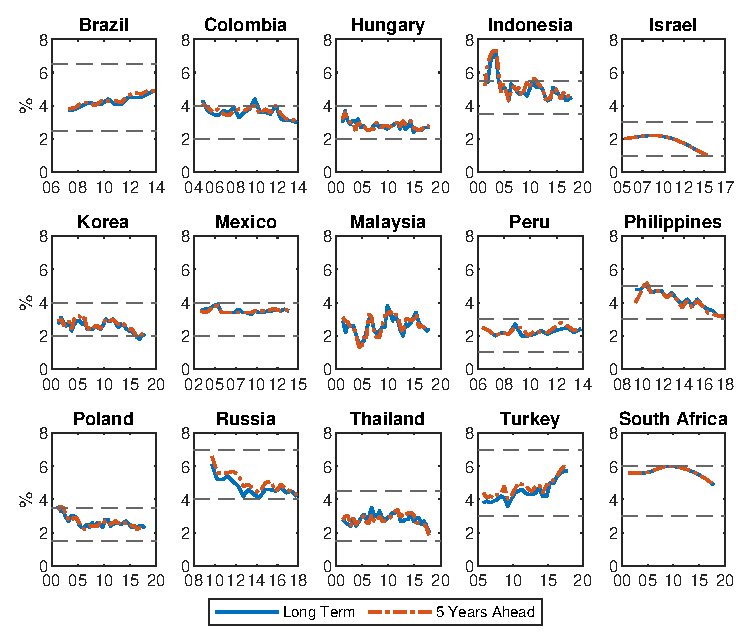
\includegraphics[trim={0cm 0cm 0cm 0cm},clip,height=0.75\textheight,width=\linewidth]{../Figures/wnCPI.eps} \\
						\end{center}
						\fignotes{This figure plots the 5-years ahead (dashed line) and the 5- to 10-years ahead or long-term (solid line) average consumer price inflation forecasts against the survey date. For Israel and South Africa, the figure shows the inflation trend, see appendix \ref{sec:trendinf}. Where applicable, the figure includes the most recent upper and lower bounds for the domestic inflation target; for Russia, since it updated its target range almost yearly since early 2000s, the plotted band shows the highest and lowest bounds since 2009.}
					\end{minipage}
				\end{center}
			\end{figure}
		\end{landscape}
	}
	
	\begin{landscape}
		\begin{figure}[tbph]
			\caption{Inflation Trend and Long-Horizon Forecast for Inflation} \label{fig:CPI_ILSZAR}
			\begin{center}								% center the minipage on the line
				\begin{minipage}{0.9\linewidth}
					\begin{center}							% center the figure inside the minipage
						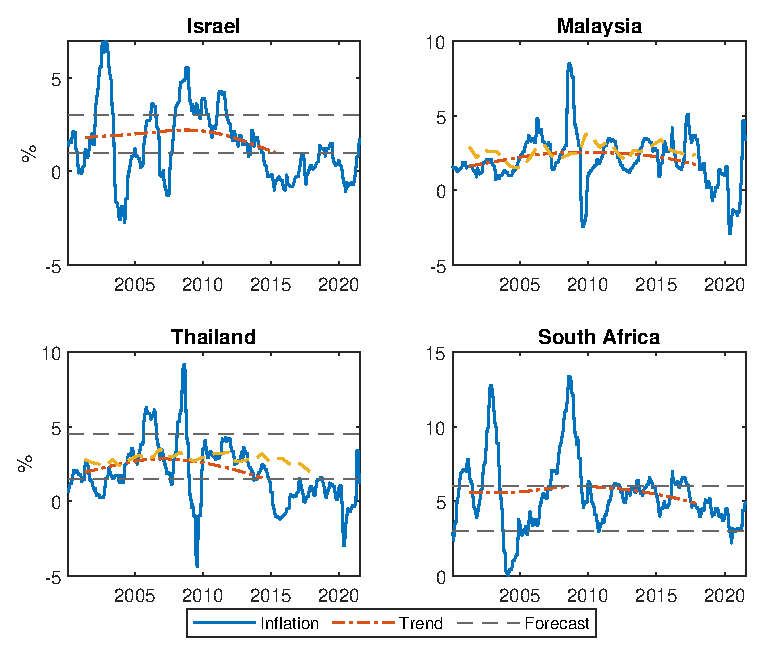
\includegraphics[trim={0cm 0cm 0cm 0cm},clip,height=0.8\textheight,width=1\textwidth]{../Figures/CPI_ILSZAR.eps} \\
					\end{center}
					\fignotes{This figure plots the consumer price inflation (solid line), inflation trend based on the Hodrick--Prescott filter (dash-dotted line) and long-term inflation forecast (dashed line). The figure includes the the most recent upper and lower bounds for the domestic inflation target.}
				\end{minipage}
			\end{center}
		\end{figure}
	\end{landscape}
	
	
	\renewcommand\thefigure{\thesection.\arabic{figure}}
	\renewcommand\thetable{\thesection.\arabic{table}}
	\section{Assessment of Yield Components} \label{sec:assessment}
	\setcounter{figure}{0}
	\setcounter{table}{0}
	\setcounter{footnote}{0}
	\setcounter{equation}{0}
	
	This appendix assesses each component and the robustness of the decomposition.
	
	\subsection{Average Expected Future Short Rate}
	Figure \ref{fig:bsl_yP_scbp} shows that the model-implied 10-year average expected future short rate aligns reasonably well with the (inferred) long-term forecast for the short rate, even though the model does not rely too much on surveys given the conservative value for \(\sigma_s\) of 75 basis points.\footnote{The results in the paper are based on this conservative value but, as a reference, when \(\sigma_s\) is estimated, its average value across all emerging markets is 31 basis points.} In contrast, when no survey data are used in the estimation, the model-implied expectations are weakly connected to the forecasts. 
	
	\afterpage{
		\begin{landscape}
			\begin{figure}[tbph]
				\caption{Long-Horizon Forecast vs. Model-Implied 10-Year Average Expected Future Short Rate} \label{fig:bsl_yP_scbp}
				\begin{center}								% center the minipage on the line
					\begin{minipage}{0.9\linewidth}
						\begin{center}							% center the figure inside the minipage
							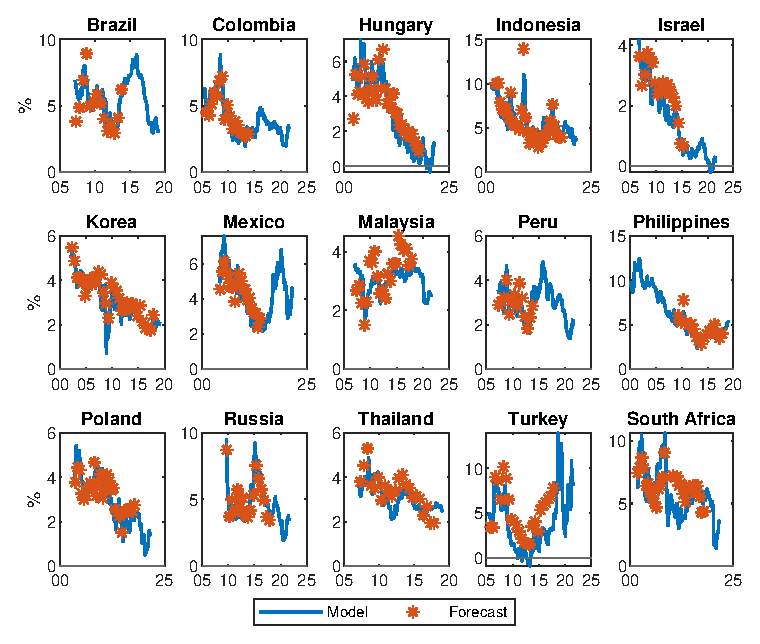
\includegraphics[trim={0cm 0cm 0cm 0cm},clip,height=0.8\textheight,width=\linewidth]{../Figures/bsl_yP_scbp.eps} \\
						\end{center}
						\fignotes{This figure plots the (inferred) long-horizon forecast of the domestic short-term interest rate (asterisk) and the 10-year average expected future short-term interest rate implied by the model (solid line).}
					\end{minipage}
				\end{center}
			\end{figure}
		\end{landscape}
	}
	
	\subsection{Term Premium} \label{sec:TP}
	Using synthetic yields (and surveys) in the estimation results in a genuine term premium, clean of credit risk. A simple test for the model-implied term premium is to compare it against a model-free measure. The survey-based term premium is the difference between the \textit{synthetic} yield and the short rate forecast over the same horizon. Since the model-implied expectations track the short rate forecasts closely (see figure \ref{fig:bsl_yP_scbp}), the two measures comove positively, with an average correlation of 0.52 for the 10-year maturity. %corr dtp120m scbp120m if em -> (obs=346) 0.5219
	
	An alternative test is to assess whether the term premium is related to inflation uncertainty. \cite{Wright:2011} documents a downward trend in the term premia of advanced economies and argues that it owes in part to a reduction in inflation uncertainty. That relationship should be particularly relevant in emerging markets given that their inflation tends to be higher and more volatile than in advanced economies \citep{HaKoseOhnsorge:2019}. To test this hypothesis, I run the following panel regressions 
	\begin{equation*}
	\eqpanelUCSV ,
	\end{equation*}
	in which the dependent variable \(\tau_{\idxspnl}\) is the model-implied term premium at different maturities, \(\alpha_{\idxi}\) are country fixed effects, \(\sigma^{\pi}_{\idxspnl}\) is a measure of inflation uncertainty, \(GDP_{\idxspnl}\) is the domestic real GDP growth to control for the business cycle, and \(u_{\idxspnl}\) is the error term. Following \cite{Wright:2011}, the measure of inflation uncertainty is the standard deviation of the permanent component of inflation in the Stock--Watson unobserved components stochastic volatility (UCSV) model, estimated using quarterly data for each country. The UCSV model assumes that inflation has permanent and transitory components subject to uncorrelated shocks that vary over time. I use the Driscoll--Kraay estimator to test for significance; the Pesaran test of cross-sectional independence is rejected in all cases at the 1\% significance level. 
	%Lag selection based on Newey \& West(1994) “plug-in” estimator. Automatic lag selection in covariance matrix estimation, Review of Economic Studies 61: 631–653.
	
	Table \ref{tab:tpucsv} shows that the term premium and the standard deviation of the permanent component are positively associated. The relationship is significant for medium- and long-term maturities, and the relevance increases with maturity. The results become stronger after controlling for the business cycle. Although this specification might be subject to econometric problems, since it involves persistent variables and ignores measurement error, the results are aligned with the view that the term premium in emerging markets compensates investors for bearing inflation uncertainty.
	
	\afterpage{
		\begin{normalsize}
			\begin{landscape}
				\begin{table}
					\begin{center}
						\caption{Term Premia and Inflation Volatility} \label{tab:tpucsv}
						\begin{threeparttable}
							\begin{tabularx}{0.95\linewidth}{l*{10}C}
								\toprule
								&\multicolumn{2}{c}{6 Months}               &\multicolumn{2}{c}{1 Year}                 &\multicolumn{2}{c}{2 Years}                &\multicolumn{2}{c}{5 Years}                &\multicolumn{2}{c}{10 Years}               \\\cmidrule(lr){2-3}\cmidrule(lr){4-5}\cmidrule(lr){6-7}\cmidrule(lr){8-9}\cmidrule(lr){10-11}
								UCSV-Perm           &        43.1         &        37.8         &        26.6         &        38.6         &        18.9         &        42.2\sym{*}  &        31.3\sym{**} &        66.9\sym{***}&        61.9\sym{***}&       108.0\sym{***}\\
								&      (30.2)         &      (27.5)         &      (19.9)         &      (25.4)         &      (12.8)         &      (18.5)         &      (9.42)         &      (13.0)         &      (12.3)         &      (15.7)         \\
								GDP Growth          &                     &       -0.53         &                     &      -0.069         &                     &        0.73         &                     &        1.32         &                     &        0.86         \\
								&                     &      (1.46)         &                     &      (1.66)         &                     &      (1.31)         &                     &      (1.20)         &                     &      (2.14)         \\\midrule
								Fixed Effects       &         Yes         &         Yes         &         Yes         &         Yes         &         Yes         &         Yes         &         Yes         &         Yes         &         Yes         &         Yes         \\
								Lags                &           3         &           3         &           3         &           3         &           3         &           3         &           3         &           3         &           3         &           3         \\
								No. Countries       &          15         &          14         &          15         &          14         &          15         &          14         &          15         &          14         &          15         &          14         \\
								Observations        &         980         &         885         &         980         &         885         &         980         &         885         &         980         &         885         &         980         &         885         \\
								\(R^{2}\)           &        0.02         &        0.01         &        0.01         &        0.01         &        0.01         &        0.02         &        0.02         &        0.07         &        0.05         &        0.13         \\
								\bottomrule
								\addlinespace[.75ex]
							\end{tabularx}
							\tabnote{This table reports the slope coefficients of panel data regressions of the model-implied term premia for different maturities on the standard deviation of the permanent component of inflation according to the UCSV model (UCSV-Perm) and GDP growth. The sample includes quarterly data for 15 countries starting in 2000:I and ending in 2021:II. Term premia are expressed in basis points. GDP growth is expressed in percent. Driscoll--Kraay standard errors are in parenthesis; the lag length up to which the residuals may be autocorrelated is indicated. *, **, *** asterisks respectively indicate significance at the 10\%, 5\% and 1\% level.}
						\end{threeparttable}
					\end{center}
				\end{table}
			\end{landscape}
		\end{normalsize}
	}
	
	Lastly, a negative term premium is not an advanced economy phenomenon. A term premium becomes negative when investors see bonds as hedges and are therefore willing to give up some investment returns. This is a well-known phenomenon for advanced economies, especially after the global financial crisis. Figure \ref{fig:bsl_tp_ts} shows that the term premium in some emerging markets has also been negative. In particular, strong macroeconomic fundamentals in Asia increased the demand for LC bonds since 2011 \citep{IMFWB:2020}, which partly explains the negative term premia seen for Korea, Malaysia, the Philippines and Thailand. 
	
	\afterpage{
		\begin{landscape}
			\begin{figure}[tbph]
				\caption{Term Structure of Term Premia} \label{fig:bsl_tp_ts}
				\begin{center}								% center the minipage on the line
					\begin{minipage}{0.9\linewidth}
						\begin{center}							% center the figure inside the minipage
							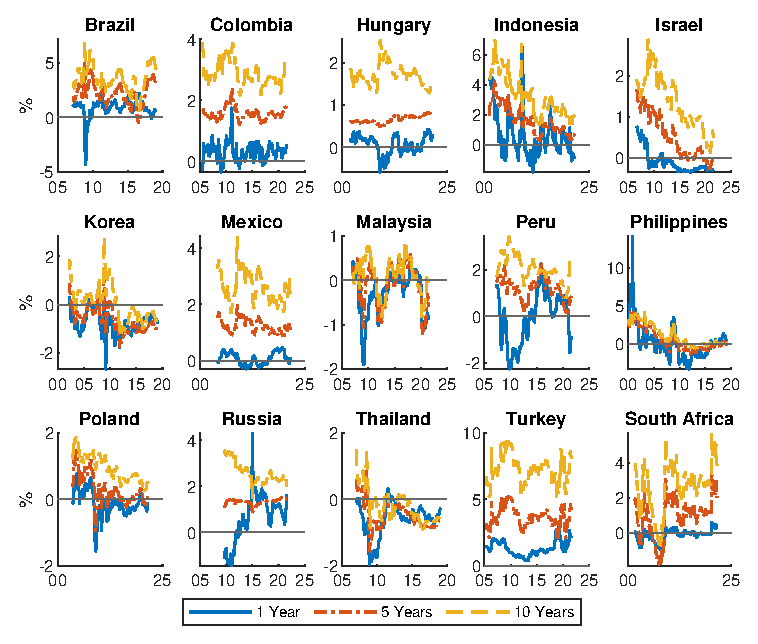
\includegraphics[trim={0cm 0cm 0cm 0cm},clip,height=0.8\textheight,width=\linewidth]{../Figures/bsl_tp_ts.eps} \\
						\end{center}
						\fignotes{This figure plots the model-implied term premium for different maturities: 1 year (solid line), 5 years (dashed line) and 10 years (dash-dotted line).}
					\end{minipage}
				\end{center}
			\end{figure}
		\end{landscape}
	}
	
	\subsection{Credit Risk Compensation} \label{sec:CRC}
	The dynamics of the credit risk compensation (i.e., the nominal-synthetic spread) are in line with the LC credit spread reported by \cite{DuSchreger:2016JoF}; for the 10-year maturity, the average correlation between the two measures is 0.97. They show that the spread captures sovereign credit risk and that is highly correlated with the CDS of the respective country. 
	
	The nominal-synthetic spread, however, is an imperfect measure of sovereign credit risk. One caveat is that, although the unconditional mean of the spread is positive (see table \ref{tab:dcmpstats}), there have been episodes in which it turns negative. These situations can reflect financial market frictions \citep{DuSchreger:2016JoF}, including market segmentation and short selling constraints. Since a negative credit risk compensation is unrealistic, for the analysis it is set to zero when it turns negative in the data. Nevertheless, those episodes are brief and rare, so allowing the spread to be negative does not change the conclusions of the analysis in section \ref{sec:analysis}. 
	
	The nominal-synthetic spread may also be capturing things other than credit risk. In every yield decomposition, the fitting error is left in one of the components. In the three-part decomposition described in section \ref{sec:YCmodel}, the fitting error is left in the nominal-synthetic spread since the spread is computed using the fitted synthetic yields. Notwithstanding, the fitting error is relatively small; on average across emerging markets, it represents only 6\% of the spread, so it is unlikely that it materially influences the dynamics of the spread. Similarly, although other factors might as well be captured by the spread, they are also likely to be small and to vary slowly over time. 
	
	On balance, the spread is a valid measure of credit risk that is far from perfect, but is definitely better than ignoring it. Otherwise, estimates of the term premium would be contaminated with credit risk. In fact, the main benefit of using synthetic yields is that the term premium so obtained is genuine in the sense that it is `clean' of credit risk. More broadly, the term premium is clean of all that is captured by the nominal-synthetic spread. Table \ref{tab:dcmpstats} and figure \ref{fig:ny_dcmp} show that the role of the credit risk compensation in explaining yield variation is non-negligible, and thus it matters which curve is used (nominal or synthetic) when decomposing the yields of emerging markets. 
	
	Given that both the term premium and the credit risk compensation help explain yield variation in emerging markets, a natural question is whether and how they are related. However, while the term premium compensates investors for bearing the uncertainty that interest rates might suddenly change, the credit risk compensation actually rewards them for two things: for the \textit{expected} loss owing to default and for bearing the \textit{uncertainty} that defaults might be larger than expected. Therefore, interpreting any correlation between the term premium and the credit risk compensation is not straightforward, and attempting to decompose the latter into those two parts is beyond the scope of the paper. 
	
	\subsection{Robustness}
	The yield decomposition provides valuable insights as long as it is reliable. To assess its robustness, I compute the standard errors for each component using the delta method. Specifically, since each yield component \(\cmpnt\) is a function of the parameters \(\theta\) in the model, \(\cmpnt = g(\params) \), its distribution is calculated based on the following
	\begin{equation*}
	\asydstr ,
	\end{equation*}
	in which \(\Vasy\) is the asymptotic covariance matrix of the estimator \(\widehat{\params}\) and \(\Jacobian\) is the Jacobian matrix of partial derivatives calculated numerically. \(\Vasy\) is estimated using the sample Hessian estimator \(\widehat{\Vasy} = \widehat{\Hessian}^{-1} \), for which the second derivative matrix of the log-likelihood function evaluated at the optimum, \(\widehat{\Hessian}\), is also calculated numerically using the individual log densities. Notice that \(\widehat{\Hessian}\) can also be estimated using the joint log density since \(\widehat{\Hessian} = - \sampleHindiv = - \sampleHjoint\). 
	
	Although there is uncertainty in both the parameters and the pricing factors after the estimation, the effect of uncertainty associated with the pricing factors on each component is usually small.\footnote{ To verify this, at each period, I compute the standard errors by pre- and post-multiplying the variance of the pricing factors (generated by the Kalman filter) by the respective factor loadings for the fitted yields, the average expected future short rate and the term premium. In all cases, the average standard error (over time and across countries) is less than 9 basis points for emerging markets, and less than 3 basis points for advanced economies.} Therefore, when applying the delta method, I assume that the pricing factors are known with certainty. Figures \ref{fig:bsl_tp_CI_10y_V1} and \ref{fig:bsl_cr_CI_10y_V1} display the term premium and the credit risk compensation along with their confidence bands. The bands are narrow, which illustrates the benefits of using survey data during the estimation. Therefore, in line with the findings of \cite{Guimaraes:2014} for the U.S. and the U.K., surveys help to obtain robust decompositions of emerging market yields.
	
	\begin{landscape}
		\begin{figure}[tbph]
			\caption{The 10-Year Term Premium of Emerging Markets} \label{fig:bsl_tp_CI_10y_V1}
			\begin{center}								% center the minipage on the line
				\begin{minipage}{0.9\linewidth}
					\begin{center}							% center the figure inside the minipage
						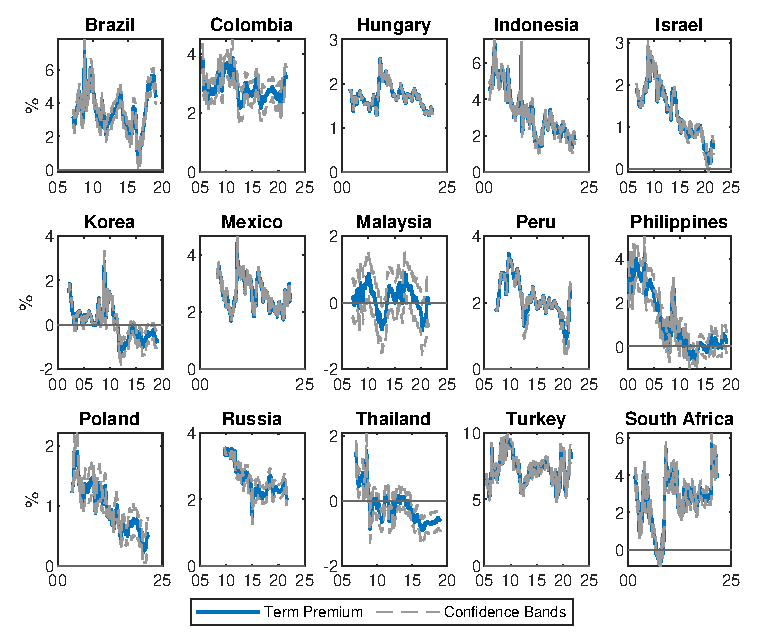
\includegraphics[trim={0cm 0cm 0cm 0cm},clip,height=0.8\textheight,width=\linewidth]{../Figures/bsl_tp_CI_10y_V1.eps} \\
					\end{center}
					\fignotes{This figure plots the model-implied 10-year term premium (solid line) along with 2-standard-error confidence intervals (dashed lines). The standard errors are estimated using the delta method. The covariance matrix is estimated using the sample Hessian estimator calculated numerically from the joint log density.}
				\end{minipage}
			\end{center}
		\end{figure}
		
		\begin{figure}[tbph]
			\caption{The 10-Year Credit Risk Compensation of Emerging Markets} \label{fig:bsl_cr_CI_10y_V1}
			\begin{center}								% center the minipage on the line
				\begin{minipage}{0.9\linewidth}
					\begin{center}							% center the figure inside the minipage
						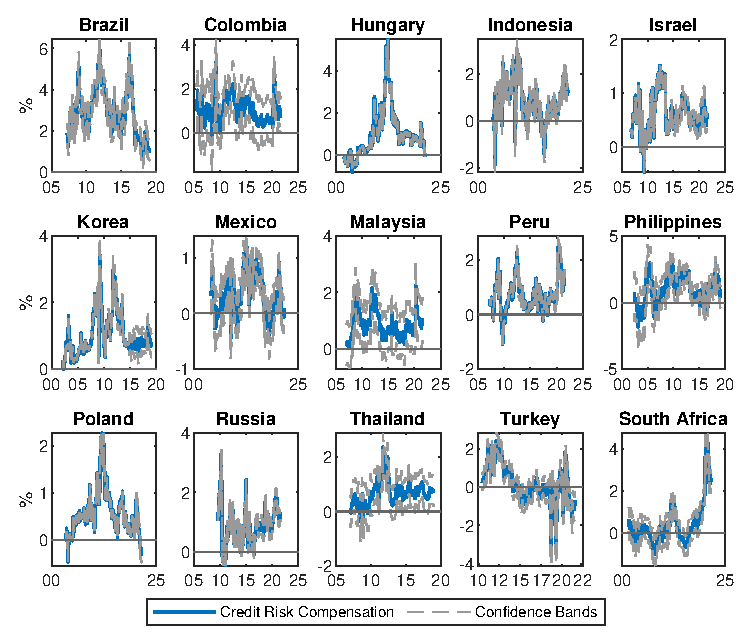
\includegraphics[trim={0cm 0cm 0cm 0cm},clip,height=0.8\textheight,width=\linewidth]{../Figures/bsl_cr_CI_10y_V1.eps} \\
					\end{center}
					\fignotes{This figure plots the model-implied 10-year credit risk compensation (solid line) along with 2-standard-error confidence intervals (dashed lines). The standard errors are estimated using the delta method. The covariance matrix is estimated using the sample Hessian estimator calculated numerically from the joint log density.}
				\end{minipage}
			\end{center}
		\end{figure}
	\end{landscape}
	
	
	\renewcommand\thefigure{\thesection.\arabic{figure}}
	\section{Comovement of Yields} \label{sec:comovement}
	\setcounter{figure}{0}
	
	This appendix shows that the long end of the yield curves of emerging markets comoves relatively more than the short end, that synthetic yields comove relatively more than nominal yields, and that the components comove similarly. 
	
	Two indicators help in assessing the comovement of yields. One approach is to use rolling correlations of daily yield changes. Another approach is to use the connectedness index of \cite{DieboldYilmaz:2014}, which assesses shares of forecast error variation in a country's yields due to shocks arising elsewhere; the index ranges from 0 to 100\%. 
	
	The long-term yields of emerging markets comove relatively more than short-term ones, yet local factors remain relevant. Figures \ref{fig:rolling_ts} and \ref{fig:dy_index_ts} use each indicator to capture the comovement of the nominal yields of emerging markets and advanced economies at different maturities. Both figures exhibit the same patterns. In particular, the long-term yields of emerging markets became more connected after the global financial crisis, and more so since the 2013 taper tantrum; whereas those of advanced economies have been more connected since the beginning of the sample period. Moreover, regardless of the indicator, the level of comovement among the long-term yields of emerging markets is less than half relative to advanced economies, suggesting that local investors remain key holders of their long-term bonds and that shocks to the yields are mainly idiosyncratic. The low connectedness among emerging market yields supports estimating the term structure models for their yield curves separately rather than jointly. 
	
	Synthetic yields comove relatively more than nominal yields. Figure \ref{subfig:dyindex10ynomsyn} compares the connectedness index for the nominal and synthetic yields of emerging markets. The level of the index for synthetic yields tends to be higher than for nominal yields, suggesting that the credit risk component is more idiosyncratic. 
	
	The components of emerging market yields comove similarly. Figure \ref{subfig:dyindex10ydcmp} compares the connectedness index of their components. They all comove similarly, although the expected future short rate comoves slightly more over the sample period, suggesting that the monetary stance of some emerging markets tends to be aligned. 
	
	\begin{figure}[tbph]
		\caption{Comovement of Yield Curves: Rolling Correlations} \label{fig:rolling_ts}
		\begin{center}
			\begin{minipage}{0.9\linewidth}
				\begin{center}
					\begin{subfigure}[t]{\linewidth}
						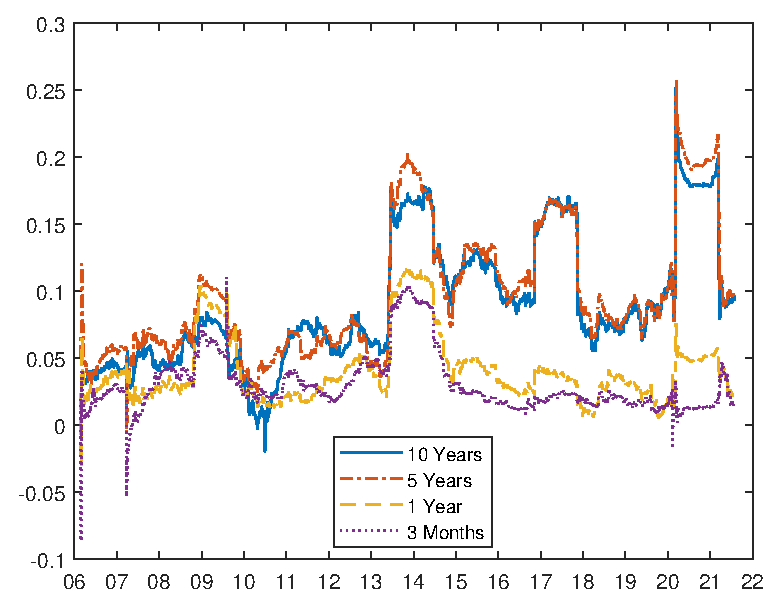
\includegraphics[trim={0cm 0cm 0cm 0cm},clip,height=0.38\textheight,width=\linewidth]{../Figures/rolling_dn_data.eps} \\
						\vspace{-0.37cm}
						\caption{Emerging Markets} \label{subfig:rolling_tsEM}
						\vspace{0.4cm}
					\end{subfigure}
					
					\begin{subfigure}[t]{\linewidth}
						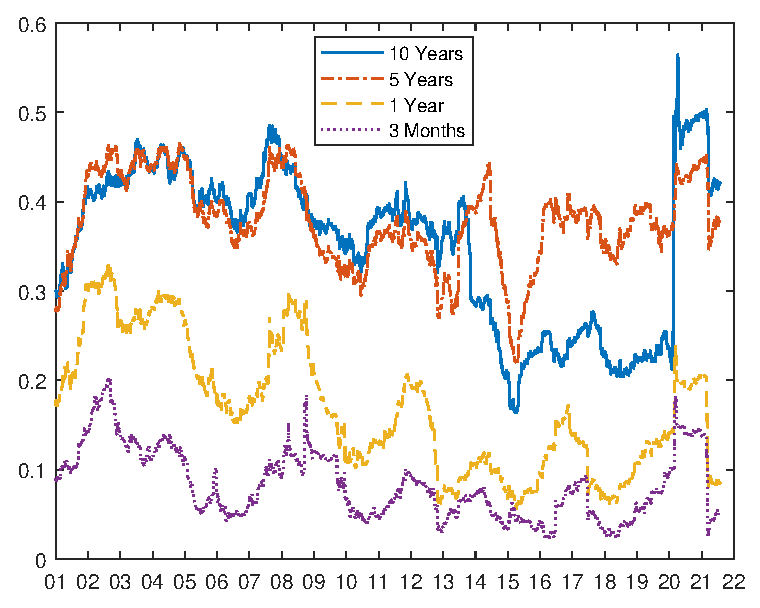
\includegraphics[trim={0cm 0cm 0cm 0cm},clip,height=0.38\textheight,width=\linewidth]{../Figures/rolling_dn_data_AE.eps} \\
						\vspace{-0.37cm}
						\caption{Advanced Economies} \label{subfig:rolling_tsAE}
						\vspace{0.4cm}
					\end{subfigure}
					
				\end{center}
				\vspace{-0.45cm}
				\fignotes{This figure plots one-year rolling correlation coefficients of daily changes in the nominal yields of emerging markets (panel a) and advanced economies (panel b) averaged across country pairs for different maturities: 10 years (solid line), 5 years (dash-dotted line), 1 year (dashed line), and 3 months (dotted line).}
			\end{minipage}
		\end{center}
	\end{figure}
	
	\begin{figure}[tbph]
		\caption{Comovement of Yield Curves: Connectedness Index} \label{fig:dy_index_ts}
		\begin{center}
			\begin{minipage}{0.9\linewidth}
				\begin{center}
					\begin{subfigure}[t]{\linewidth}
						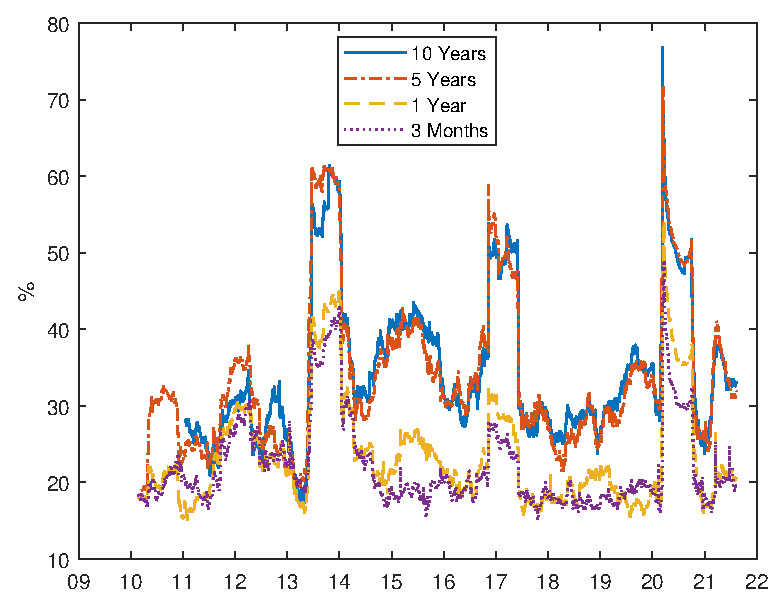
\includegraphics[trim={0cm 0cm 0cm 0cm},clip,height=0.38\textheight,width=\linewidth]{../Figures/dy_index_dn_data.eps} \\
						\vspace{-0.37cm}
						\caption{Emerging Markets} \label{subfig:dy_index_tsEM}
						%						\vspace{0.4cm}
					\end{subfigure}
					
					\begin{subfigure}[t]{\linewidth}
						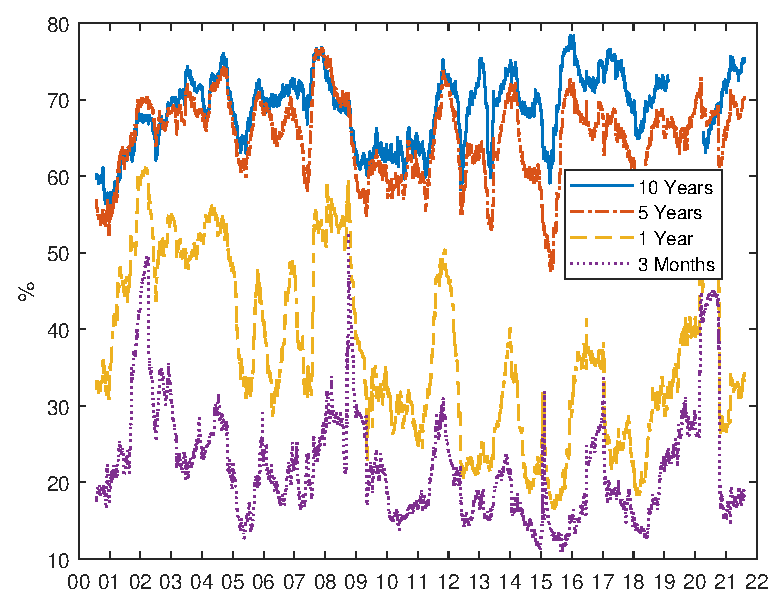
\includegraphics[trim={0cm 0cm 0cm 0cm},clip,height=0.38\textheight,width=\linewidth]{../Figures/dy_index_dn_data_AE.eps} \\
						\vspace{-0.37cm}
						\caption{Advanced Economies} \label{subfig:dy_index_tsAE}
						\vspace{0.2cm}
					\end{subfigure}
					
				\end{center}
				\vspace{-0.45cm}
				\fignotes{This figure plots the connectedness index of \cite{DieboldYilmaz:2014} for the nominal yields of emerging markets (panel a) and advanced economies (panel b) for different maturities: 10 years (solid line), 5 years (dash-dotted line), 1 year (dashed line), and 3 months (dotted line). The index is obtained using a VAR(1), with a forecast horizon of 10 days and a rolling window of 150 days for the daily changes of the nominal yields at each maturity.}
			\end{minipage}
		\end{center}
	\end{figure}
	
	\begin{figure}[tbph]
		\caption{Connectedness of 10-Year Yields and Components} \label{fig:dyindex10y}
		\begin{center}
			\begin{minipage}{0.9\linewidth}
				\begin{center}
					\begin{subfigure}[t]{\linewidth}
						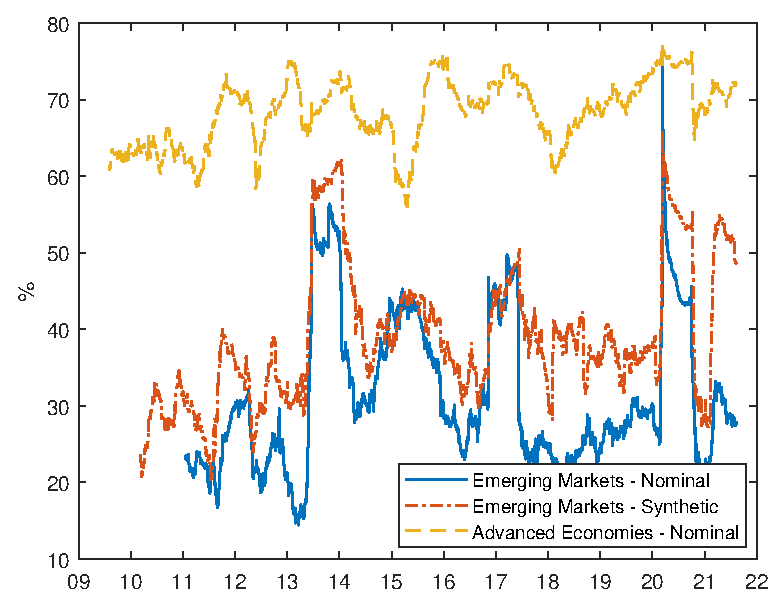
\includegraphics[trim={0cm 0cm 0cm 0cm},clip,height=0.33\textheight,width=\linewidth]{../Figures/dy_index10y_nomsyn.eps} \\
						\vspace{-0.35cm}
						\caption{Nominal and Synthetic Yields} \label{subfig:dyindex10ynomsyn}
						\vspace{0.4cm}
					\end{subfigure}
					
					\begin{subfigure}[t]{\linewidth}
						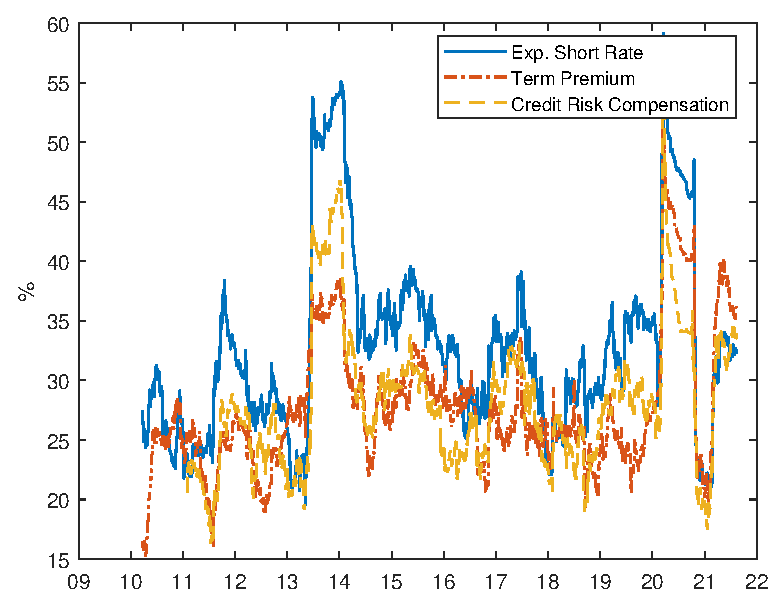
\includegraphics[trim={0cm 0cm 0cm 0cm},clip,height=0.33\textheight,width=\linewidth]{../Figures/dy_index10y_dcmp.eps} \\
						\vspace{-0.35cm}
						\caption{Nominal Yield Components} \label{subfig:dyindex10ydcmp}
					\end{subfigure}
				\end{center}
				\fignotes{This figure plots the connectedness index of \cite{DieboldYilmaz:2014} for 10-year yields. 
					Panel (a) compares the connectedness index of nominal (solid line) and synthetic (dash-dotted line) yields of emerging markets and the nominal (dashed line) yields of advanced economies. Panel (b) compares the connectedness index of each component of the nominal yields of emerging markets: the expected future short rate (solid line), the term premium (dash-dotted line) and the credit risk compensation (dashed line). The index for some components has a shorter history because its computation requires a balanced panel and the components do not start on the same date (e.g., the construction of the synthetic curves does not involve nominal yields). The index is obtained using a VAR(1), with a forecast horizon of 10 days and a rolling window of 150 days for the daily changes of the 10-year yields and their components.}
			\end{minipage}
		\end{center}
	\end{figure}
	
	\newpage
	
	%---------------------------------------------------------------
	% Figures and Tables
	%---------------------------------------------------------------
	\renewcommand{\thetable}{\thesection.\arabic{table}}
	\section{Supplementary Tables} \label{sec:AppTables}
	\setcounter{table}{0}
	
	\begin{normalsize}
		\begin{table}[!h]
			\begin{center}
				\caption{Drivers of the Emerging Market 5-Year Nominal Yield and Its Components} \label{tab:ycdcmp5y}
				\begin{threeparttable}
					\begin{tabularx}{0.95\linewidth}{l*{6}C}
						\toprule
						&\multicolumn{1}{c}{Nominal}&\multicolumn{1}{c}{E. Short Rate}&\multicolumn{1}{c}{Term Premium}&\multicolumn{1}{c}{Credit Risk}\\\cmidrule(lr){2-2}\cmidrule(lr){3-3}\cmidrule(lr){4-4}\cmidrule(lr){5-5}
						U.S. Term Premium   &        1.31\sym{***}&        0.95\sym{***}&        0.58\sym{***}&       -0.25\sym{*}  \\
						&      (0.15)         &      (0.12)         &      (0.07)         &      (0.12)         \\
						U.S. E. Short Rate  &        0.06         &        0.20\sym{***}&        0.01         &       -0.17\sym{***}\\
						&      (0.05)         &      (0.04)         &      (0.03)         &      (0.04)         \\
						Local Policy Rate   &        0.44\sym{***}&        0.56\sym{***}&       -0.08\sym{***}&       -0.00         \\
						&      (0.02)         &      (0.03)         &      (0.01)         &      (0.02)         \\
						Inflation           &       10.06\sym{***}&        4.33         &        3.49\sym{**} &        2.58         \\
						&      (2.30)         &      (2.71)         &      (1.29)         &      (1.67)         \\
						Unemployment        &       14.20\sym{***}&        0.83         &        5.69\sym{**} &        7.53\sym{***}\\
						&      (2.65)         &      (2.67)         &      (1.99)         &      (1.76)         \\
						LC per USD (Std.)   &       32.72\sym{***}&       30.89\sym{***}&       18.95\sym{***}&      -12.92\sym{**} \\
						&      (5.69)         &      (4.87)         &      (2.48)         &      (4.22)         \\
						Log(VIX)            &       52.05\sym{***}&       -6.76         &        9.55         &       49.41\sym{***}\\
						&      (9.12)         &     (13.19)         &      (5.69)         &     (10.16)         \\
						Log(EPU U.S.)       &        6.51         &       -7.07         &        3.02         &        9.08\sym{*}  \\
						&      (4.97)         &      (4.32)         &      (1.84)         &      (3.97)         \\
						Log(EPU Global)     &      -56.23\sym{***}&      -27.38\sym{*}  &      -16.93\sym{*}  &      -13.46         \\
						&     (15.43)         &     (11.16)         &      (7.62)         &      (9.09)         \\
						Global Ind. Prod.   &        1.85\sym{*}  &       -1.46         &        1.08\sym{***}&        2.22\sym{*}  \\
						&      (0.79)         &      (0.96)         &      (0.29)         &      (0.87)         \\\midrule
						Fixed Effects       &         Yes         &         Yes         &         Yes         &         Yes         \\
						Lags                &           4         &           4         &           4         &           4         \\
						No. Countries       &          15         &          15         &          15         &          15         \\
						Observations        &        2493         &        2493         &        2493         &        2493         \\
						\(R^{2}\)           &        0.76         &        0.77         &        0.20         &        0.24         \\
						\bottomrule
						\addlinespace[.75ex]
					\end{tabularx}
					\tabnote{This table reports the estimated slope coefficients of panel data regressions of the 5-year nominal yield and its components (expected short rate, term premium and credit risk compensation) on selected explanatory variables. The sample includes monthly data for 15 emerging markets starting in 2000:1 and ending in 2021:7. The dependent variables are expressed in basis points. The explanatory variables are the U.S. term premium and the U.S. expected short rate according to \cite{KimWright:2005} with the same maturity as the dependent variables, the policy rate, domestic inflation and unemployment rates, the standardized exchange rate (LC per USD), the log of the VIX, the log of the U.S. and global economic policy uncertainty indexes based on \cite{BakerBloomDavis:2016}, the global economic activity index of \cite{Hamilton:2021}. Driscoll--Kraay standard errors in parenthesis; lag length up to which the residuals may be autocorrelated is indicated. *, **, *** asterisks respectively indicate significance at the 10\%, 5\% and 1\% level.}
				\end{threeparttable}
			\end{center}
		\end{table}
	\end{normalsize}
	
	\begin{normalsize}
		\begin{table}
			\begin{center}
				\caption{Drivers of the Emerging Market 1-Year Nominal Yield and Its Components} \label{tab:ycdcmp1y}
				\begin{threeparttable}
					\begin{tabularx}{0.95\linewidth}{l*{6}C}
						\toprule
						&\multicolumn{1}{c}{Nominal}&\multicolumn{1}{c}{E. Short Rate}&\multicolumn{1}{c}{Term Premium}&\multicolumn{1}{c}{Credit Risk}\\\cmidrule(lr){2-2}\cmidrule(lr){3-3}\cmidrule(lr){4-4}\cmidrule(lr){5-5}
						U.S. Term Premium   &        2.16\sym{***}&        2.15\sym{***}&       -0.14         &       -0.07         \\
						&      (0.32)         &      (0.38)         &      (0.25)         &      (0.30)         \\
						U.S. E. Short Rate  &       -0.01         &        0.02         &        0.07\sym{***}&       -0.12\sym{***}\\
						&      (0.03)         &      (0.04)         &      (0.02)         &      (0.03)         \\
						Local Policy Rate   &        0.72\sym{***}&        0.75\sym{***}&        0.04\sym{**} &       -0.01         \\
						&      (0.02)         &      (0.03)         &      (0.02)         &      (0.02)         \\
						Inflation           &        6.07\sym{**} &        3.50         &        4.61\sym{*}  &        2.24         \\
						&      (2.29)         &      (3.21)         &      (1.96)         &      (1.58)         \\
						Unemployment        &        3.33         &       -0.05         &       -1.62         &        4.51\sym{**} \\
						&      (1.95)         &      (2.64)         &      (1.22)         &      (1.55)         \\
						LC per USD (Std.)   &       25.90\sym{***}&       29.37\sym{***}&       21.59\sym{***}&      -12.80\sym{**} \\
						&      (5.00)         &      (5.68)         &      (3.69)         &      (4.71)         \\
						Log(VIX)            &       34.13\sym{***}&       -4.69         &      -20.64\sym{**} &       65.56\sym{***}\\
						&      (7.00)         &     (13.90)         &      (7.07)         &     (11.42)         \\
						Log(EPU U.S.)       &        2.94         &       -4.61         &       -6.31\sym{*}  &       10.19\sym{**} \\
						&      (3.26)         &      (5.85)         &      (2.46)         &      (3.87)         \\
						Log(EPU Global)     &      -44.88\sym{***}&      -34.23\sym{**} &        1.29         &       -8.10         \\
						&     (11.84)         &     (12.77)         &      (7.86)         &      (8.89)         \\
						Global Ind. Prod.   &        2.09\sym{**} &       -2.42\sym{**} &       -0.80         &        3.72\sym{***}\\
						&      (0.66)         &      (0.91)         &      (0.68)         &      (0.71)         \\\midrule
						Fixed Effects       &         Yes         &         Yes         &         Yes         &         Yes         \\
						Lags                &           4         &           4         &           4         &           4         \\
						No. Countries       &          15         &          15         &          15         &          15         \\
						Observations        &        2493         &        2493         &        2493         &        2493         \\
						\(R^{2}\)           &        0.84         &        0.78         &        0.20         &        0.27         \\
						\bottomrule
						\addlinespace[.75ex]
					\end{tabularx}
					\tabnote{This table reports the estimated slope coefficients of panel data regressions of the 1-year nominal yield and its components (expected short rate, term premium and credit risk compensation) on selected explanatory variables. The sample includes monthly data for 15 emerging markets starting in 2000:1 and ending in 2021:7. The dependent variables are expressed in basis points. The explanatory variables are the U.S. term premium and the U.S. expected short rate according to \cite{KimWright:2005} with the same maturity as the dependent variables, the policy rate, domestic inflation and unemployment rates, the standardized exchange rate (LC per USD), the log of the VIX, the log of the U.S. and global economic policy uncertainty indexes based on \cite{BakerBloomDavis:2016}, the global economic activity index of \cite{Hamilton:2021}. Driscoll--Kraay standard errors in parenthesis; lag length up to which the residuals may be autocorrelated is indicated. *, **, *** asterisks respectively indicate significance at the 10\%, 5\% and 1\% level.}
				\end{threeparttable}
			\end{center}
		\end{table}
	\end{normalsize}
	
	\newpage
	
	
	\renewcommand\thefigure{\thesection.\arabic{figure}}
	\section{Supplementary Figures} \label{sec:AppFigures}
	\setcounter{figure}{0}
	
	\afterpage{
		\begin{landscape}
			\begin{figure}[tbph]
				\caption{10-Year Synthetic Yields and Long-Horizon Implied Forecasts of the Short Rate} \label{fig:YLD10Y_CBP}
				\begin{center}								% center the minipage on the line
					\begin{minipage}{0.9\linewidth}
						\begin{center}							% center the figure inside the minipage
							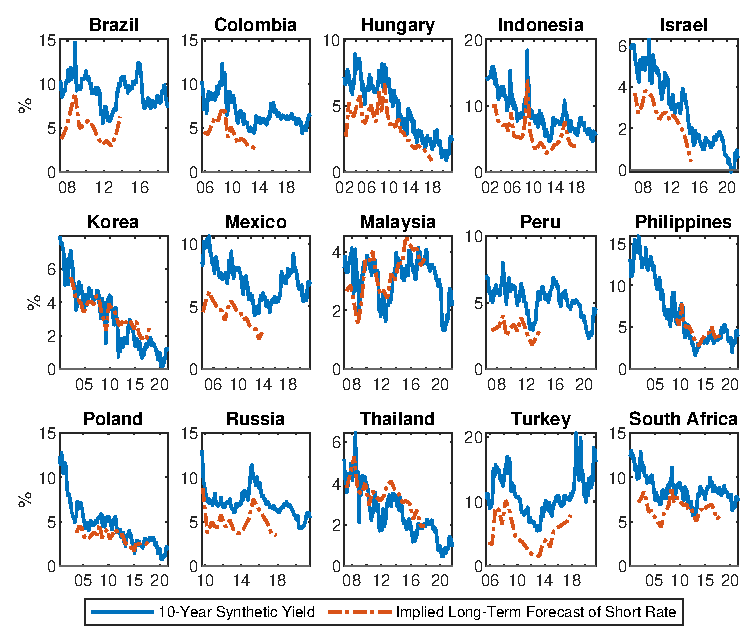
\includegraphics[trim={0cm 0cm 0cm 0cm},clip,height=0.75\textheight,width=\linewidth]{../Figures/YLD10Y_CBP.eps} \\
						\end{center}
						\fignotes{This figure plots the long-horizon implied forecast of the domestic nominal short-term interest rate (dashed line) and the 10-year synthetic yield (solid line). The implied forecast of the short rate is equal to the forecast of the U.S. real short-term interest rate corrected for a real forward premium plus the inflation forecast, see section \ref{sec:SurveyData} for details. The forecast of the U.S. real short-term rate is equal to the difference between the forecast for the three-month U.S. Treasury bill rate and the forecast for the U.S. consumer price inflation.}
					\end{minipage}
				\end{center}
			\end{figure}
		\end{landscape}
	}
	
	\afterpage{
		\begin{landscape}
			\begin{figure}[tbph]
				\caption{Model Fit: 10-Year Synthetic Yields of Emerging Markets} \label{fig:s_ylds_bsl_yQ}
				\begin{center}								% center the minipage on the line
					\begin{minipage}{0.9\linewidth}
						\begin{center}							% center the figure inside the minipage
							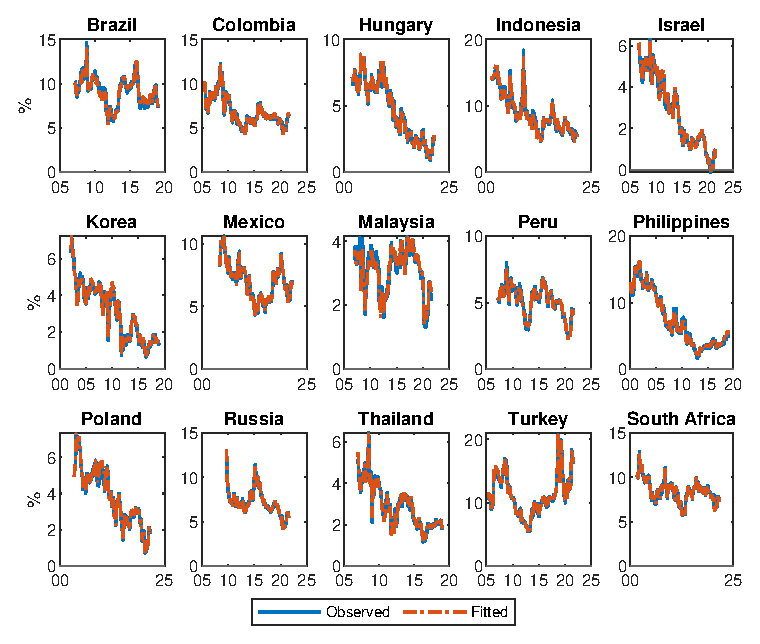
\includegraphics[trim={0cm 0cm 0cm 0cm},clip,height=0.8\textheight,width=\linewidth]{../Figures/s_ylds_bsl_yQ.eps} \\
						\end{center}
						\fignotes{This figure plots the fitted (dashed line) and the actual (solid line) 10-year synthetic yields. The fitted yields are obtained after estimating the survey-augmented affine term structure model.}
					\end{minipage}
				\end{center}
			\end{figure}
		\end{landscape}
	}
	
	\begin{landscape}
		
		\begin{figure}[tbph]
			\caption{Response of the U.S. Yield Curve to a Target Surprise} \label{fig:LPUStarget}
			\begin{center}
				\begin{minipage}{\linewidth}
					\begin{center}
						\begin{subfigure}[t]{\linewidth}
							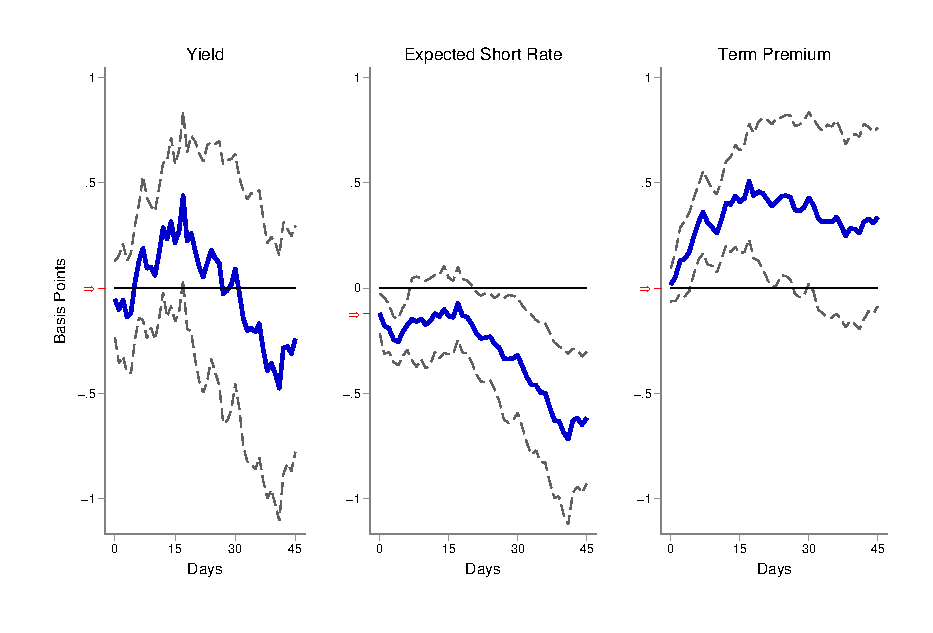
\includegraphics[trim={0cm 0cm 0cm 0cm},clip,height=0.35\textheight,width=\linewidth]{../Figures/TargetUSDnomyptp120m.eps} \\
							\vspace{-0.35cm}
							\caption{10-Year Yield} \label{subfig:LPUS10Ytarget}
							\vspace{0.4cm}
						\end{subfigure}
						
						\begin{subfigure}[t]{\linewidth}
							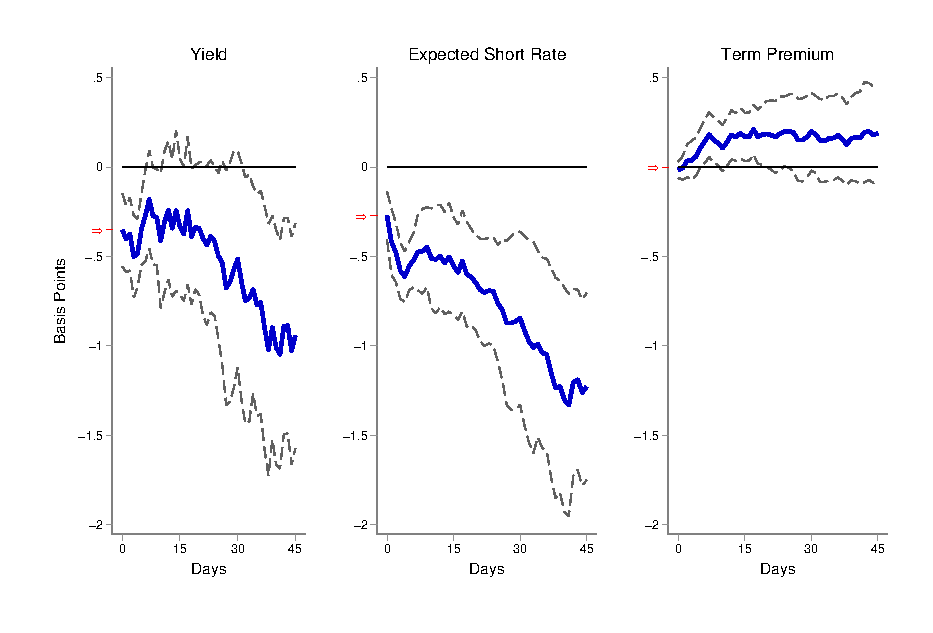
\includegraphics[trim={0cm 0cm 0cm 0cm},clip,height=0.35\textheight,width=\linewidth]{../Figures/TargetUSDnomyptp24m.eps} \\
							\vspace{-0.35cm}
							\caption{2-Year Yield} \label{subfig:LPUS2Ytarget}
						\end{subfigure}
						\vspace{-0.45cm}
					\end{center}
					\fignotes{This figure shows the response of the 10- and 2-year U.S. yields and their components to a target easing surprise of 1 basis point. U.S. yields are zero-coupon yields from \cite{GSW:2007}, and are decomposed into an expected future short-term interest rate and a term premium following \cite{KimWright:2005}. Target surprises are identified using intraday data around U.S. monetary policy announcements, see section \ref{sec:USMPS} for details. The 90\% confidence bands are based on Driscoll--Kraay standard errors.}
				\end{minipage}
			\end{center}
		\end{figure}
		
		\pagebreak[4]
		
		\begin{figure}[tbph]
			\caption{Response of the U.S. Yield Curve to a Forward Guidance Surprise: 2000-2008} \label{fig:LPUSpathPre}
			\begin{center}
				\begin{minipage}{\linewidth}
					\begin{center}
						\begin{subfigure}[t]{\linewidth}
							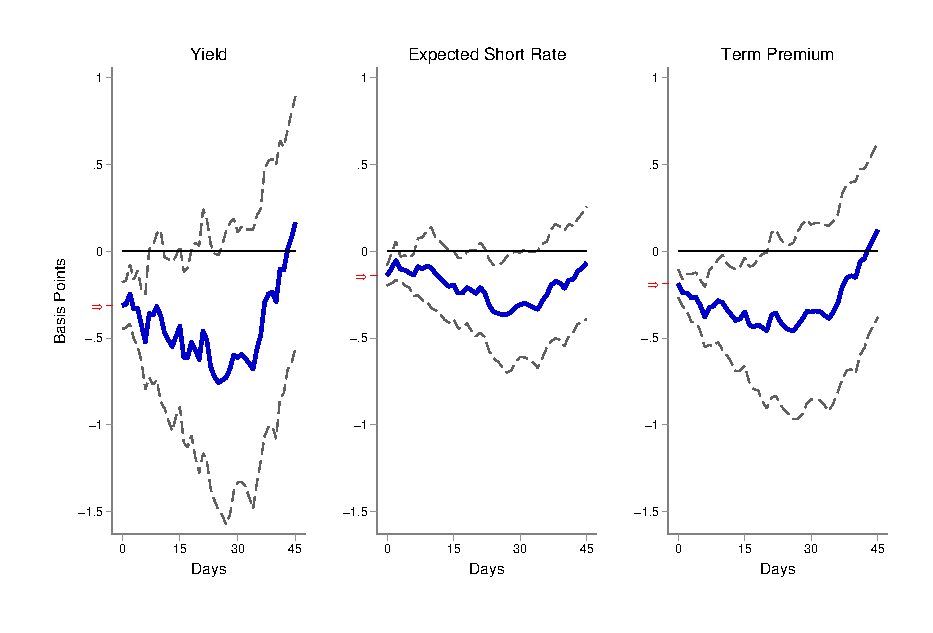
\includegraphics[trim={0cm 0cm 0cm 0cm},clip,height=0.35\textheight,width=\linewidth]{../Figures/PathUSDnomyptp120mPre.eps} \\
							\vspace{-0.35cm}
							\caption{10-Year Yield} \label{subfig:LPUS10YpathPre}
						\end{subfigure}
						
						\vspace{0.2cm}
						
						\begin{subfigure}[t]{\linewidth}
							\includegraphics[trim={0cm 0cm 0cm 0cm},clip,height=0.35\textheight,width=\linewidth]{../Figures/PathUSDnomyptp24mPre.eps} \\
							\vspace{-0.35cm}
							\caption{2-Year Yield} \label{subfig:LPUS2YpathPre}
						\end{subfigure}
						\vspace{-0.45cm}
					\end{center}
					\fignotes{This figure shows the response of the 10- and 2-year U.S. yields and their components to a forward guidance easing surprise of 1 basis point. U.S. yields are zero-coupon yields from \cite{GSW:2007}, and are decomposed into an expected future short-term interest rate and a term premium following \cite{KimWright:2005}. Forward guidance surprises are identified using intraday data around U.S. monetary policy announcements, see section \ref{sec:USMPS} for details. The 90\% confidence bands are based on Driscoll--Kraay standard errors.}
				\end{minipage}
			\end{center}
		\end{figure}
		
		\pagebreak[4]
		
		\begin{figure}[tbph]
			\caption{Response of the U.S. Yield Curve to a Forward Guidance Surprise: 2008-2019} \label{fig:LPUSpathPost}
			\begin{center}
				\begin{minipage}{\linewidth}
					\begin{center}
						\begin{subfigure}[t]{\linewidth}
							\includegraphics[trim={0cm 0cm 0cm 0cm},clip,height=0.35\textheight,width=\linewidth]{../Figures/PathUSDnomyptp120mPost.eps} \\
							\vspace{-0.35cm}
							\caption{10-Year Yield} \label{subfig:LPUS10YpathPost}
						\end{subfigure}
						
						\vspace{0.2cm}
						
						\begin{subfigure}[t]{\linewidth}
							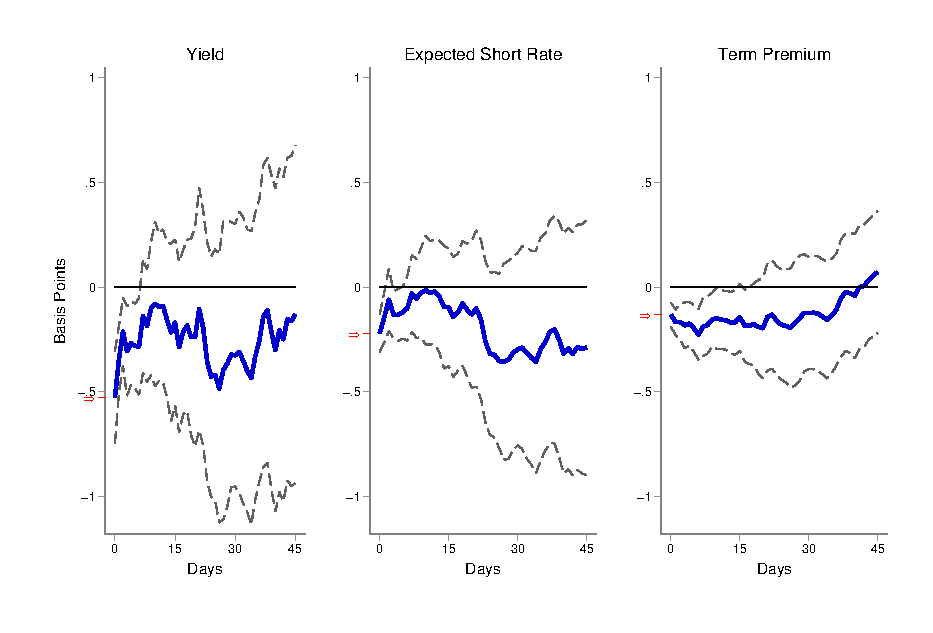
\includegraphics[trim={0cm 0cm 0cm 0cm},clip,height=0.35\textheight,width=\linewidth]{../Figures/PathUSDnomyptp24mPost.eps} \\
							\vspace{-0.35cm}
							\caption{2-Year Yield} \label{subfig:LPUS2YpathPost}
						\end{subfigure}
						\vspace{-0.45cm}
					\end{center}
					\fignotes{This figure shows the response of the 10- and 2-year U.S. yields and their components to a forward guidance easing surprise of 1 basis point. U.S. yields are zero-coupon yields from \cite{GSW:2007}, and are decomposed into an expected future short-term interest rate and a term premium following \cite{KimWright:2005}. Forward guidance surprises are identified using intraday data around U.S. monetary policy announcements, see section \ref{sec:USMPS} for details. The 90\% confidence bands are based on Driscoll--Kraay standard errors.}
				\end{minipage}
			\end{center}
		\end{figure}
		
		\pagebreak[4]
		
		\begin{figure}[tbph]
			\caption{Response of the U.S. Yield Curve to an Asset Purchase Surprise} \label{fig:LPUSlsap}
			\begin{center}
				\begin{minipage}{\linewidth}
					\begin{center}
						\begin{subfigure}[t]{\linewidth}
							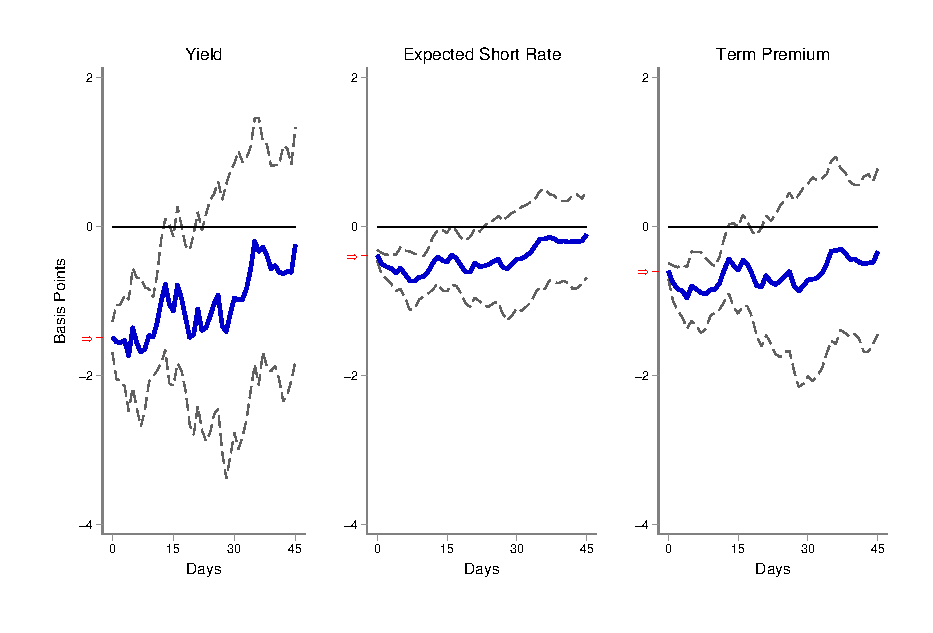
\includegraphics[trim={0cm 0cm 0cm 0cm},clip,height=0.35\textheight,width=\linewidth]{../Figures/LSAPUSDnomyptp120m.eps} \\
							\vspace{-0.35cm}
							\caption{10-Year Yield} \label{subfig:LPUS10Ylsap}
						\end{subfigure}
						
						\vspace{0.2cm}
						
						\begin{subfigure}[t]{\linewidth}
							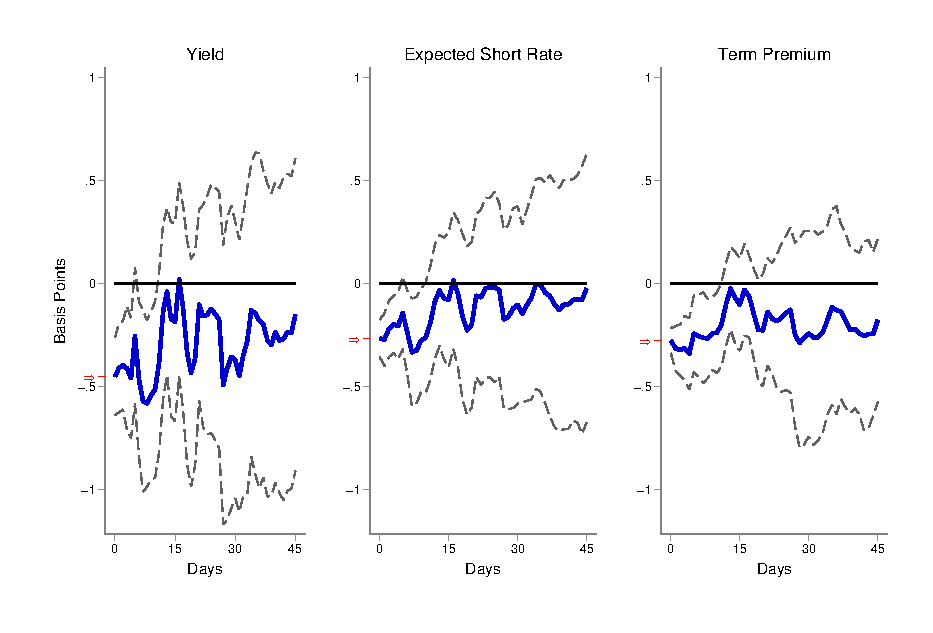
\includegraphics[trim={0cm 0cm 0cm 0cm},clip,height=0.35\textheight,width=\linewidth]{../Figures/LSAPUSDnomyptp24m.eps} \\
							\vspace{-0.35cm}
							\caption{2-Year Yield} \label{subfig:LPUS2Ylsap}
						\end{subfigure}
						\vspace{-0.45cm}
					\end{center}
					\fignotes{This figure shows the response of the 10- and 2-year U.S. yields and their components to an asset purchase easing surprise of 1 basis point. U.S. yields are zero-coupon yields from \cite{GSW:2007}, and are decomposed into an expected future short-term interest rate and a term premium following \cite{KimWright:2005}. Asset purchase surprises are identified using intraday data around U.S. monetary policy announcements, see section \ref{sec:USMPS} for details. The 90\% confidence bands are based on Driscoll--Kraay standard errors.}
				\end{minipage}
			\end{center}
		\end{figure}
		
		
		\begin{figure}[tbph]
			\caption{Response of the U.S. Yield Curve to a Forward Guidance Surprise: 2000-2019} \label{fig:LPUSpathWh}
			\begin{center}
				\begin{minipage}{\linewidth}
					\begin{center}
						\begin{subfigure}[t]{\linewidth}
							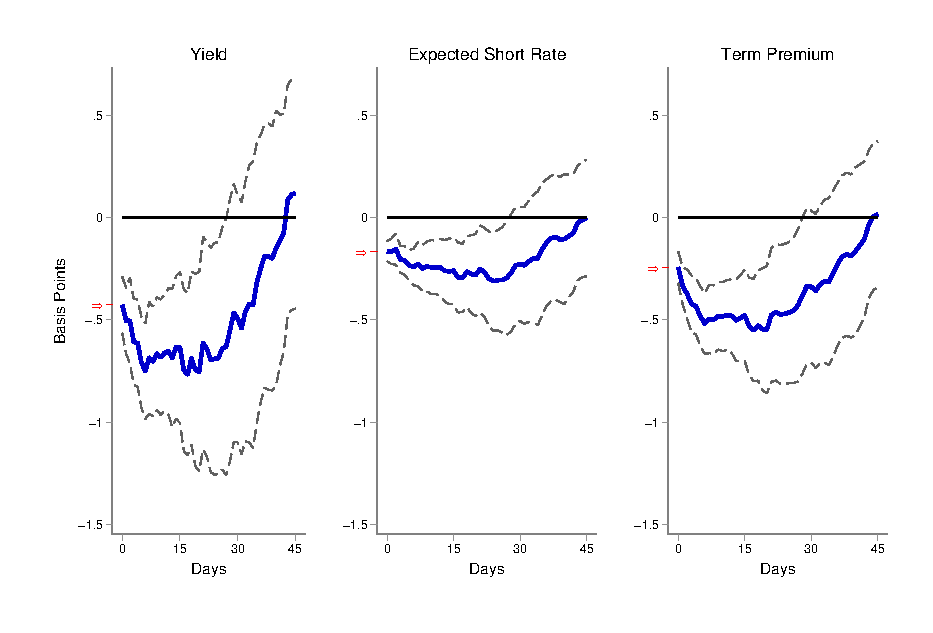
\includegraphics[trim={0cm 0cm 0cm 0cm},clip,height=0.35\textheight,width=\linewidth]{../Figures/PathUSDnomyptp120m.eps} \\
							\vspace{-0.35cm}
							\caption{10-Year Yield} \label{subfig:LPUS10YpathWh}
						\end{subfigure}
						
						\vspace{0.2cm}
						
						\begin{subfigure}[t]{\linewidth}
							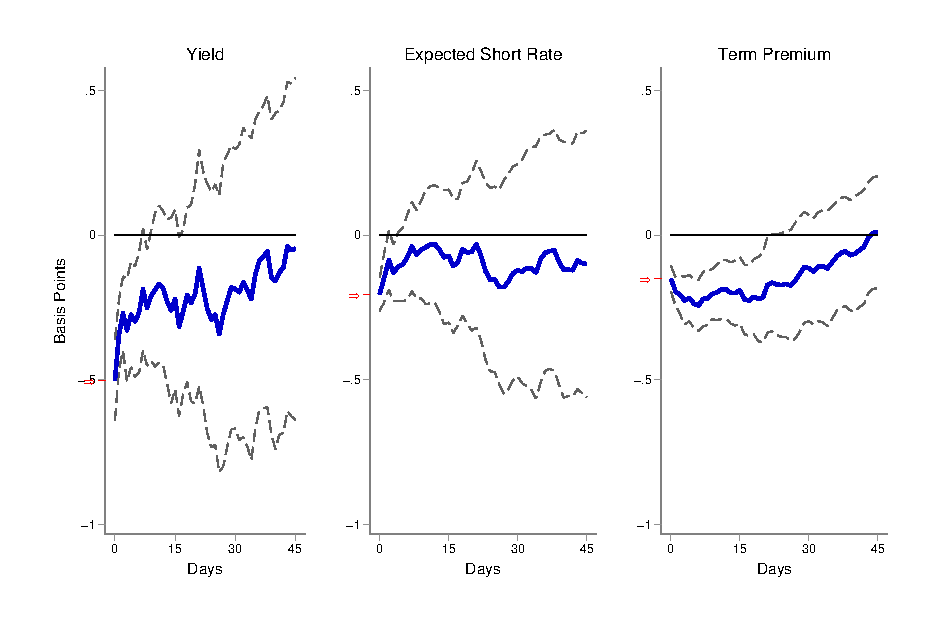
\includegraphics[trim={0cm 0cm 0cm 0cm},clip,height=0.35\textheight,width=\linewidth]{../Figures/PathUSDnomyptp24m.eps} \\
							\vspace{-0.35cm}
							\caption{2-Year Yield} \label{subfig:LPUS2YpathWh}
						\end{subfigure}
						\vspace{-0.45cm}
					\end{center}
					\fignotes{This figure shows the response of the 10- and 2-year U.S. yields and their components to a forward guidance easing surprise of 1 basis point. U.S. yields are zero-coupon yields from \cite{GSW:2007}, and are decomposed into an expected future short-term interest rate and a term premium following \cite{KimWright:2005}. Forward guidance surprises are identified using intraday data around U.S. monetary policy announcements, see section \ref{sec:USMPS} for details. The 90\% confidence bands are based on Driscoll--Kraay standard errors.}
				\end{minipage}
			\end{center}
		\end{figure}
		
	\end{landscape}
	
	
	\begin{landscape}
		
		\begin{figure}[tbph]
			\caption{Response of the 10-Year Emerging Market Yield by Region to a Target Surprise} \label{fig:LPLAEEtarget}
			\begin{center}
				\begin{minipage}{\linewidth}
					\begin{center}
						\begin{subfigure}[t]{\linewidth}
							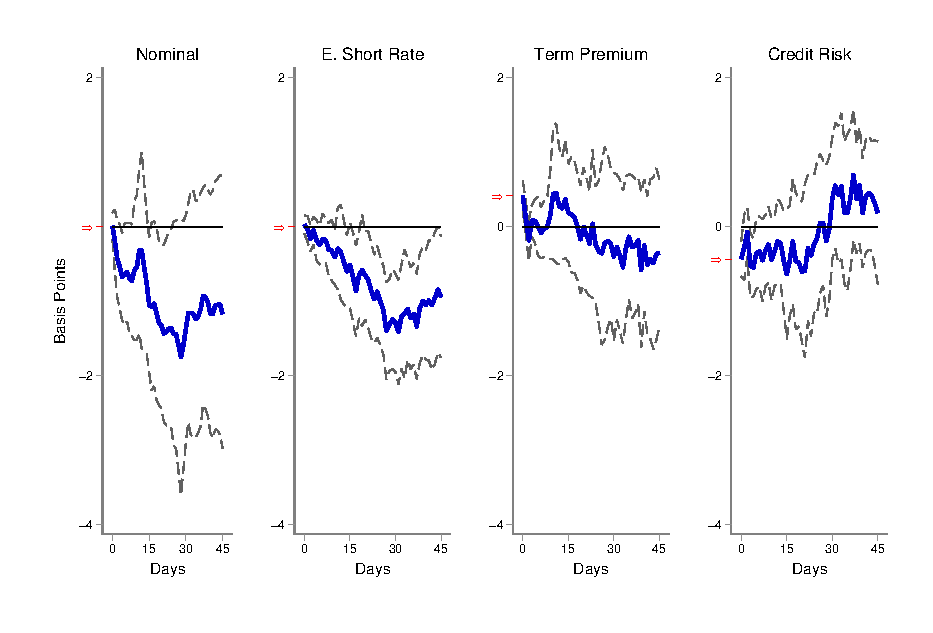
\includegraphics[trim={0cm 0cm 0cm 0cm},clip,height=0.35\textheight,width=\linewidth]{../Figures/TargetLAnomyptpphi120m.eps} \\
							\vspace{-0.35cm}
							\caption{Latin America} \label{subfig:LPLA10Ytarget}
							\vspace{0.4cm}
						\end{subfigure}
						
						\vspace{0.2cm}
						
						\begin{subfigure}[t]{\linewidth}
							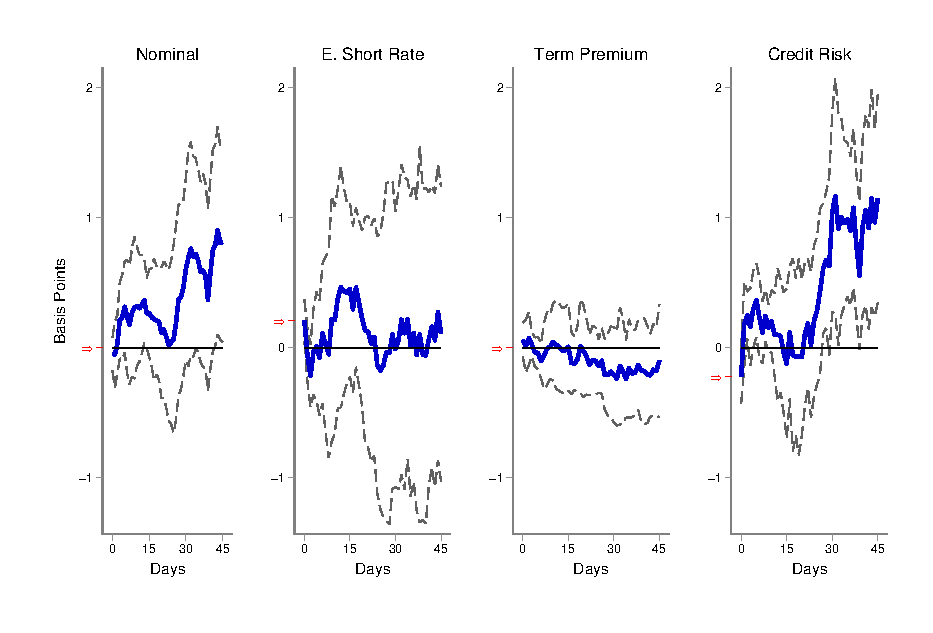
\includegraphics[trim={0cm 0cm 0cm 0cm},clip,height=0.35\textheight,width=\linewidth]{../Figures/TargetEEnomyptpphi120m.eps} \\
							\vspace{-0.35cm}
							\caption{Emerging Europe} \label{subfig:LPEE10Ytarget}
						\end{subfigure}
						\vspace{-0.45cm}
					\end{center}
					\fignotes{This figure shows the response of the 10-year emerging market nominal yields and their components by region to a target easing surprise of 1 basis point. Nominal yields are decomposed into an expected future short-term interest rate, a term premium and credit risk compensation, see section \ref{sec:Decomposition} for details. Target surprises are identified using intraday data around U.S. monetary policy announcements, see section \ref{sec:USMPS} for details. The 90\% confidence bands are based on Driscoll--Kraay standard errors.}
				\end{minipage}
			\end{center}
		\end{figure}
		
		\pagebreak[4]
		
		\begin{figure}[tbph]
			\caption{Response of the 10-Year Emerging Market Yield by Region to a Target Surprise (cont.)} \label{fig:LPEAMAtarget}
			\begin{center}
				\begin{minipage}{\linewidth}
					\begin{center}
						\begin{subfigure}[t]{\linewidth}
							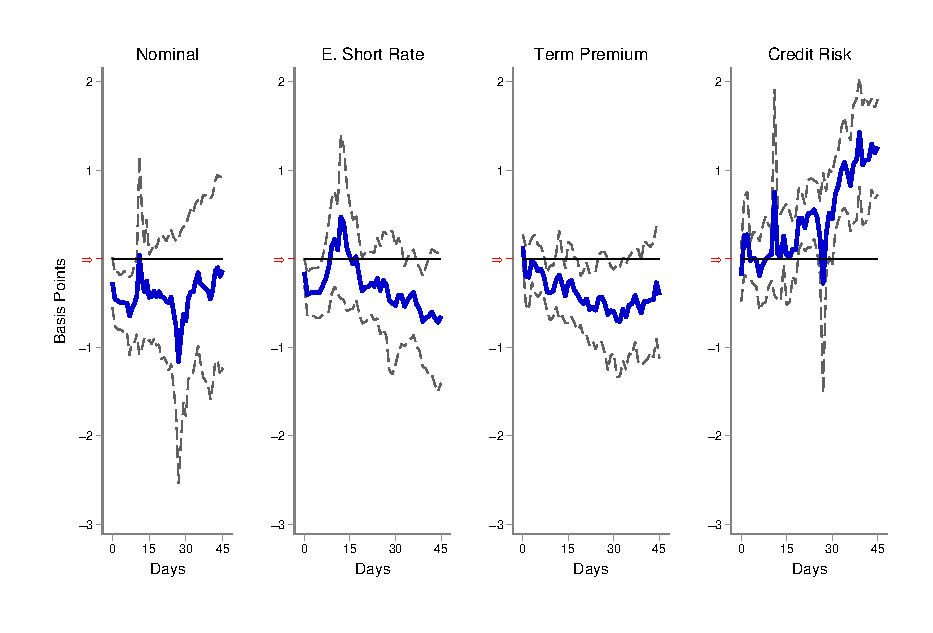
\includegraphics[trim={0cm 0cm 0cm 0cm},clip,height=0.35\textheight,width=\linewidth]{../Figures/TargetEAnomyptpphi120m.eps} \\
							\vspace{-0.35cm}
							\caption{Emerging Asia} \label{subfig:LPEA10Ytarget}
							\vspace{0.4cm}
						\end{subfigure}
						
						\vspace{0.2cm}
						
						\begin{subfigure}[t]{\linewidth}
							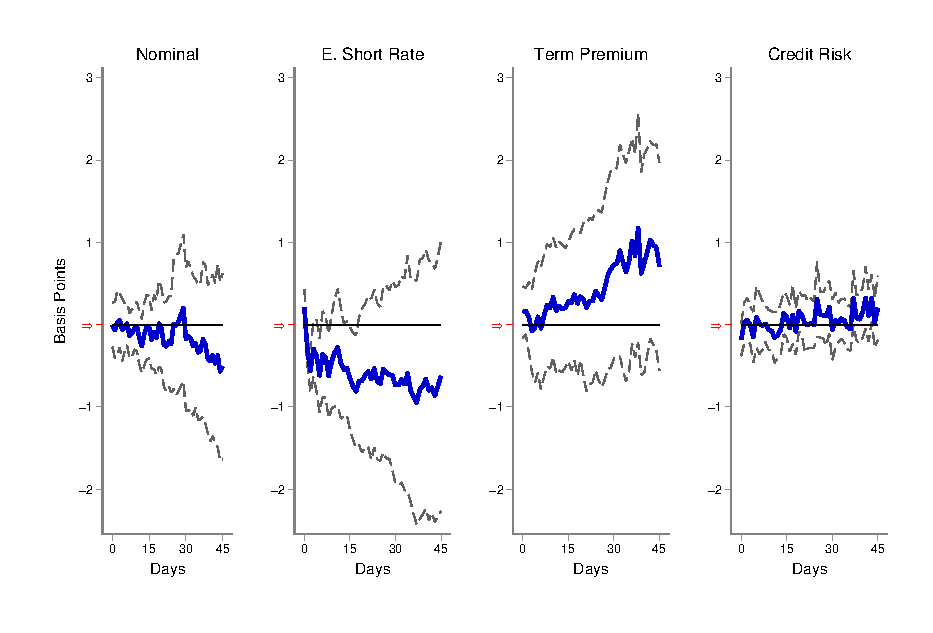
\includegraphics[trim={0cm 0cm 0cm 0cm},clip,height=0.35\textheight,width=\linewidth]{../Figures/TargetMAnomyptpphi120m.eps} \\
							\vspace{-0.35cm}
							\caption{Middle East and Africa} \label{subfig:LPMA10Ytarget}
							%						\vspace{0.4cm}
						\end{subfigure}
						\vspace{-0.45cm}
					\end{center}
					\fignotes{This figure shows the response of the 10-year emerging market nominal yields and their components by region to a target easing surprise of 1 basis point. Nominal yields are decomposed into an expected future short-term interest rate, a term premium and credit risk compensation, see section \ref{sec:Decomposition} for details. Target surprises are identified using intraday data around U.S. monetary policy announcements, see section \ref{sec:USMPS} for details. The 90\% confidence bands are based on Driscoll--Kraay standard errors.}
				\end{minipage}
			\end{center}
		\end{figure}
		
		\pagebreak[4]
		
		\begin{figure}[tbph]
			\caption{Response of the 10-Year Emerging Market Yield by Region to a Forward Guidance Surprise: 2000-2019} \label{fig:LPLAEEpath}
			\begin{center}
				\begin{minipage}{\linewidth}
					\begin{center}
						\begin{subfigure}[t]{\linewidth}
							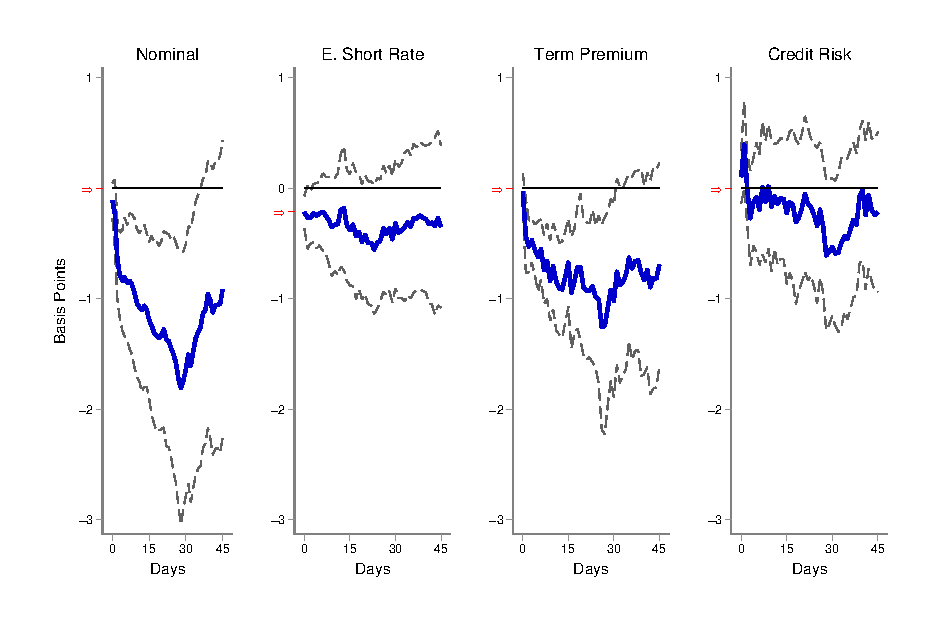
\includegraphics[trim={0cm 0cm 0cm 0cm},clip,height=0.35\textheight,width=\linewidth]{../Figures/PathLAnomyptpphi120m.eps} \\
							\vspace{-0.35cm}
							\caption{Latin America} \label{subfig:LPLA10Ypath}
						\end{subfigure}
						
						\vspace{0.2cm}
						
						\begin{subfigure}[t]{\linewidth}
							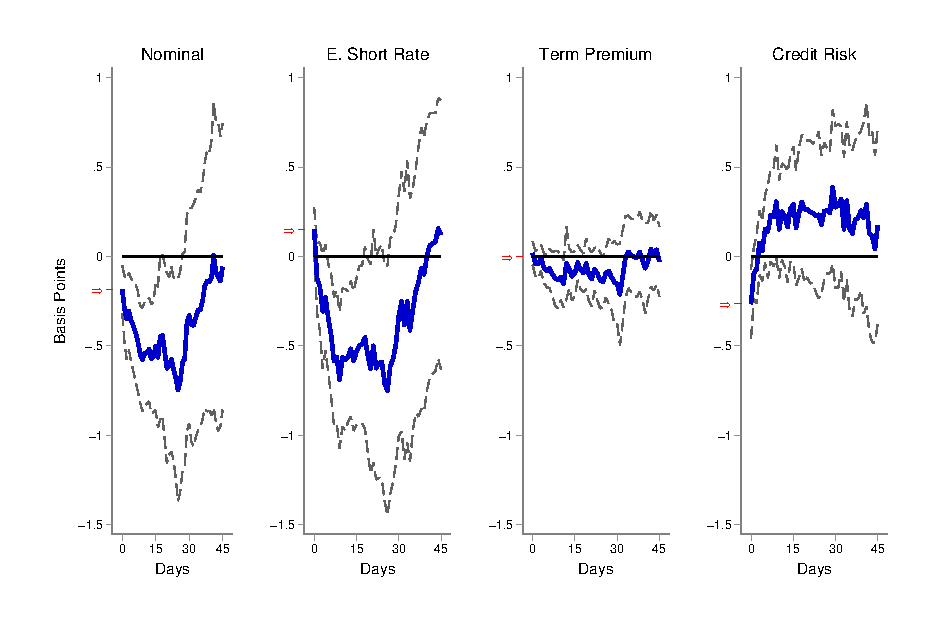
\includegraphics[trim={0cm 0cm 0cm 0cm},clip,height=0.35\textheight,width=\linewidth]{../Figures/PathEEnomyptpphi120m.eps} \\
							\vspace{-0.35cm}
							\caption{Emerging Europe} \label{subfig:LPEE10Ypath}
						\end{subfigure}
						\vspace{-0.45cm}
					\end{center}
					\fignotes{This figure shows the response of the 10-year emerging market nominal yields and their components by region to a forward guidance easing surprise of 1 basis point. Nominal yields are decomposed into an expected future short-term interest rate, a term premium and credit risk compensation, see section \ref{sec:Decomposition} for details. Forward guidance surprises are identified using intraday data around U.S. monetary policy announcements, see section \ref{sec:USMPS} for details. The 90\% confidence bands are based on Driscoll--Kraay standard errors.}
				\end{minipage}
			\end{center}
		\end{figure}
		
		\pagebreak[4]
		
		\begin{figure}[tbph]
			\caption{Response of the 10-Year Emerging Market Yield by Region to a Forward Guidance Surprise: 2000-2019 (cont.)} \label{fig:LPEAMApath}
			\begin{center}
				\begin{minipage}{\linewidth}
					\begin{center}
						\begin{subfigure}[t]{\linewidth}
							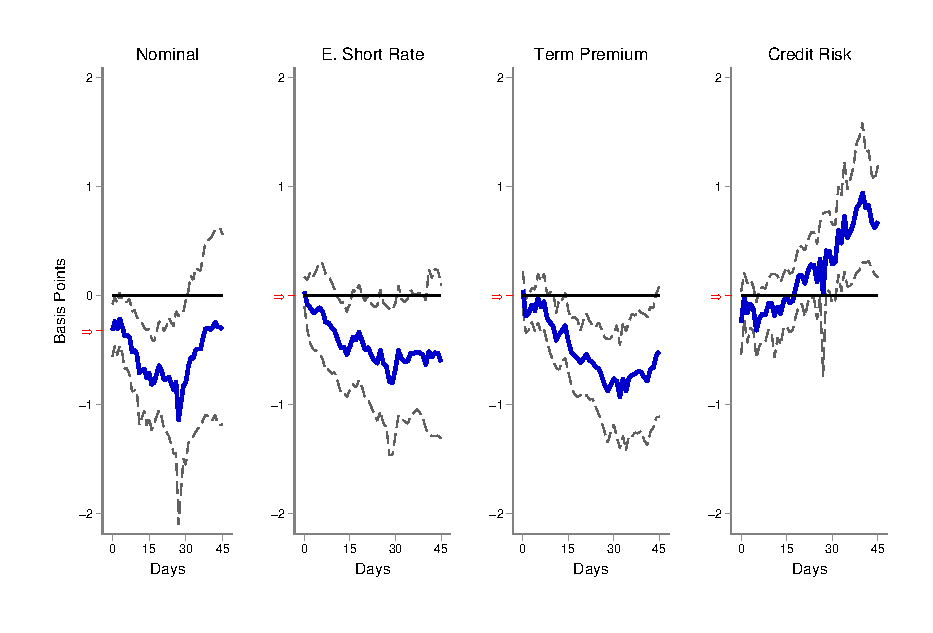
\includegraphics[trim={0cm 0cm 0cm 0cm},clip,height=0.35\textheight,width=\linewidth]{../Figures/PathEAnomyptpphi120m.eps} \\
							\vspace{-0.35cm}
							\caption{Emerging Asia} \label{subfig:LPEA10Ypath}
						\end{subfigure}
						
						\vspace{0.2cm}
						
						\begin{subfigure}[t]{\linewidth}
							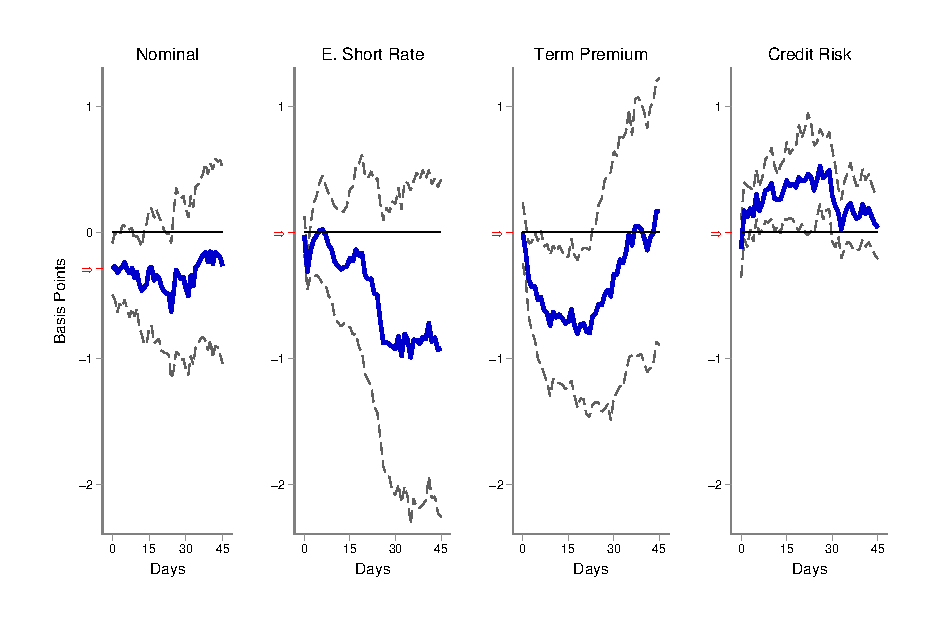
\includegraphics[trim={0cm 0cm 0cm 0cm},clip,height=0.35\textheight,width=\linewidth]{../Figures/PathMAnomyptpphi120m.eps} \\
							\vspace{-0.35cm}
							\caption{Middle East and Africa} \label{subfig:LPMA10Ypath}
						\end{subfigure}
						\vspace{-0.45cm}
					\end{center}
					\fignotes{This figure shows the response of the 10-year emerging market nominal yields and their components by region to a forward guidance easing surprise of 1 basis point. Nominal yields are decomposed into an expected future short-term interest rate, a term premium and credit risk compensation, see section \ref{sec:Decomposition} for details. Forward guidance surprises are identified using intraday data around U.S. monetary policy announcements, see section \ref{sec:USMPS} for details. The 90\% confidence bands are based on Driscoll--Kraay standard errors.}
				\end{minipage}
			\end{center}
		\end{figure}
		
		\pagebreak[4]
		
		\begin{figure}[tbph]
			\caption{Response of the 10-Year Emerging Market Yield by Region to an Asset Purchase Surprise} \label{fig:LPLAEElsap}
			\begin{center}
				\begin{minipage}{\linewidth}
					\begin{center}
						\begin{subfigure}[t]{\linewidth}
							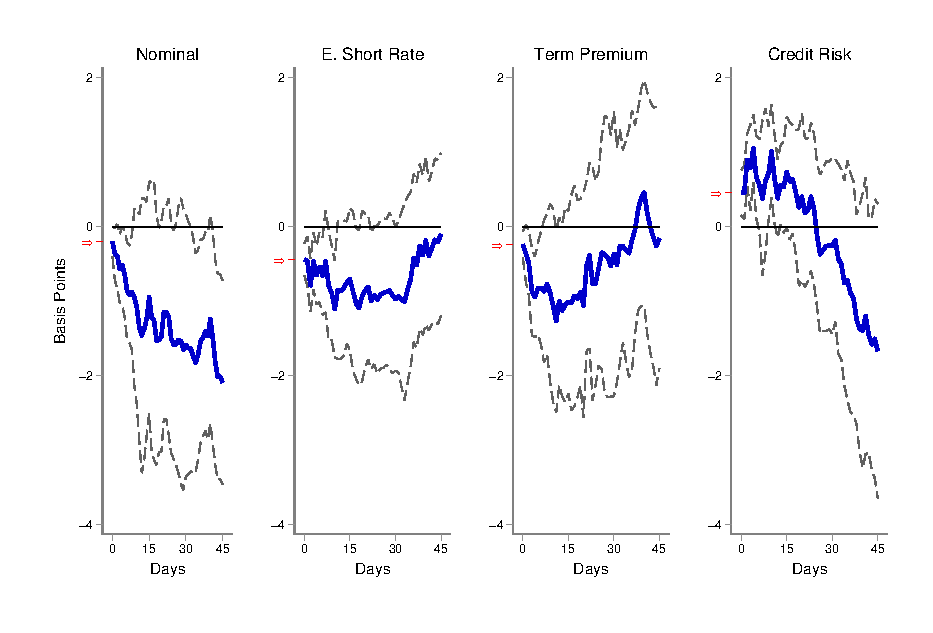
\includegraphics[trim={0cm 0cm 0cm 0cm},clip,height=0.35\textheight,width=\linewidth]{../Figures/LSAPLAnomyptpphi120m.eps} \\
							\vspace{-0.35cm}
							\caption{Latin America} \label{subfig:LPLA10Ylsap}
						\end{subfigure}
						
						\vspace{0.2cm}
						
						\begin{subfigure}[t]{\linewidth}
							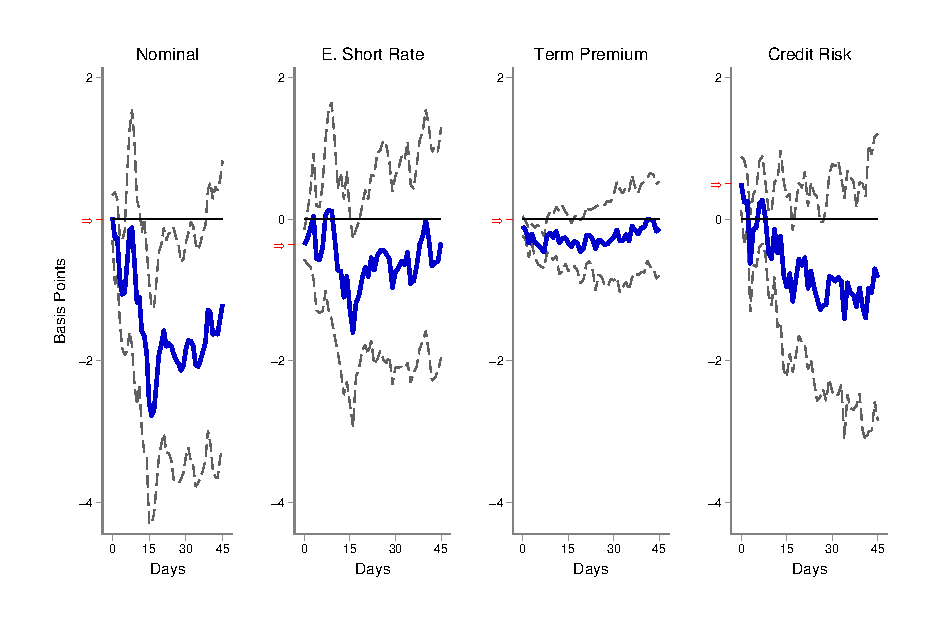
\includegraphics[trim={0cm 0cm 0cm 0cm},clip,height=0.35\textheight,width=\linewidth]{../Figures/LSAPEEnomyptpphi120m.eps} \\
							\vspace{-0.35cm}
							\caption{Emerging Europe} \label{subfig:LPEE10Ylsap}
						\end{subfigure}
						\vspace{-0.45cm}
					\end{center}
					\fignotes{This figure shows the response of the 10-year emerging market nominal yields and their components by region to an asset purchase easing surprise of 1 basis point. Nominal yields are decomposed into an expected future short-term interest rate, a term premium and credit risk compensation, see section \ref{sec:Decomposition} for details. Asset purchase surprises are identified using intraday data around U.S. monetary policy announcements, see section \ref{sec:USMPS} for details. The 90\% confidence bands are based on Driscoll--Kraay standard errors.}
				\end{minipage}
			\end{center}
		\end{figure}
		
		\pagebreak[4]
		
		\begin{figure}[tbph]
			\caption{Response of the 10-Year Emerging Market Yield by Region to an Asset Purchase Surprise (cont.)} \label{fig:LPEAMAlsap}
			\begin{center}
				\begin{minipage}{\linewidth}
					\begin{center}
						\begin{subfigure}[t]{\linewidth}
							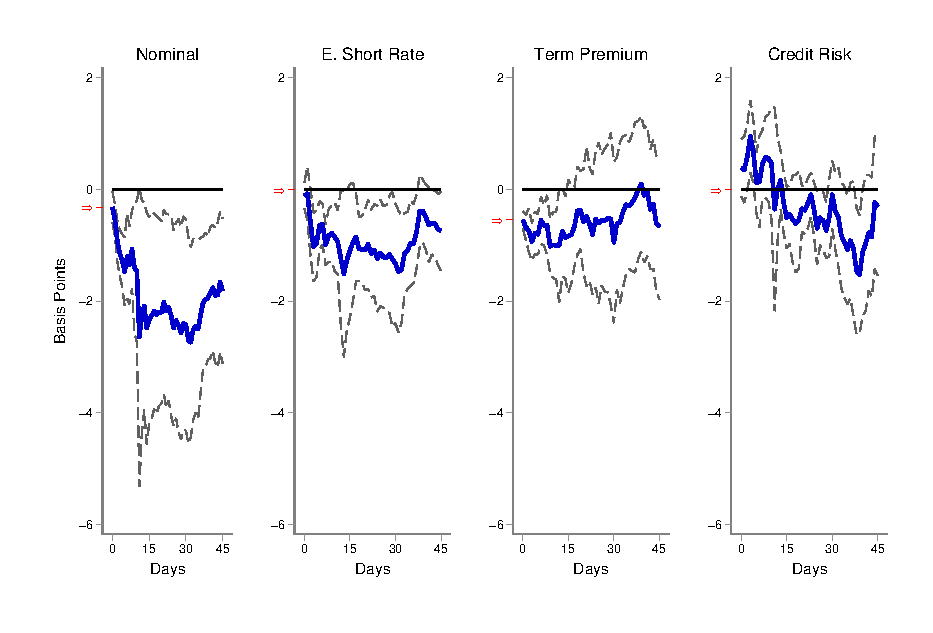
\includegraphics[trim={0cm 0cm 0cm 0cm},clip,height=0.35\textheight,width=\linewidth]{../Figures/LSAPEAnomyptpphi120m.eps} \\
							\vspace{-0.35cm}
							\caption{Emerging Asia} \label{subfig:LPEA10Ylsap}
						\end{subfigure}
						
						\vspace{0.2cm}
						
						\begin{subfigure}[t]{\linewidth}
							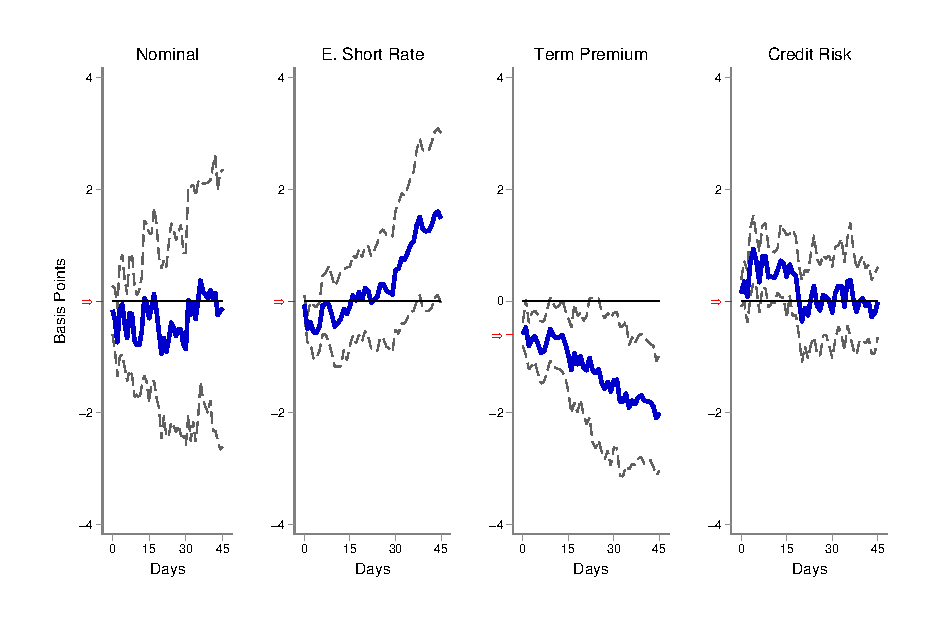
\includegraphics[trim={0cm 0cm 0cm 0cm},clip,height=0.35\textheight,width=\linewidth]{../Figures/LSAPMAnomyptpphi120m.eps} \\
							\vspace{-0.35cm}
							\caption{Middle East and Africa} \label{subfig:LPMA10Ylsap}
						\end{subfigure}
						\vspace{-0.45cm}
					\end{center}
					\fignotes{This figure shows the response of the 10--year emerging market nominal yields and their components by region to an asset purchase easing surprise of 1 basis point. Nominal yields are decomposed into an expected future short-term interest rate, a term premium and credit risk compensation, see section \ref{sec:Decomposition} for details. Asset purchase surprises are identified using intraday data around U.S. monetary policy announcements, see section \ref{sec:USMPS} for details. The 90\% confidence bands are based on Driscoll--Kraay standard errors.}
				\end{minipage}
			\end{center}
		\end{figure}
		
		
		\begin{figure}[tbph]
			\caption{Response of Emerging Market Yield Curves to a Forward Guidance Surprise: 2000-2019} \label{fig:LPEMpathWh}
			\begin{center}
				\begin{minipage}{\linewidth}
					\begin{center}
						\begin{subfigure}[t]{\linewidth}
							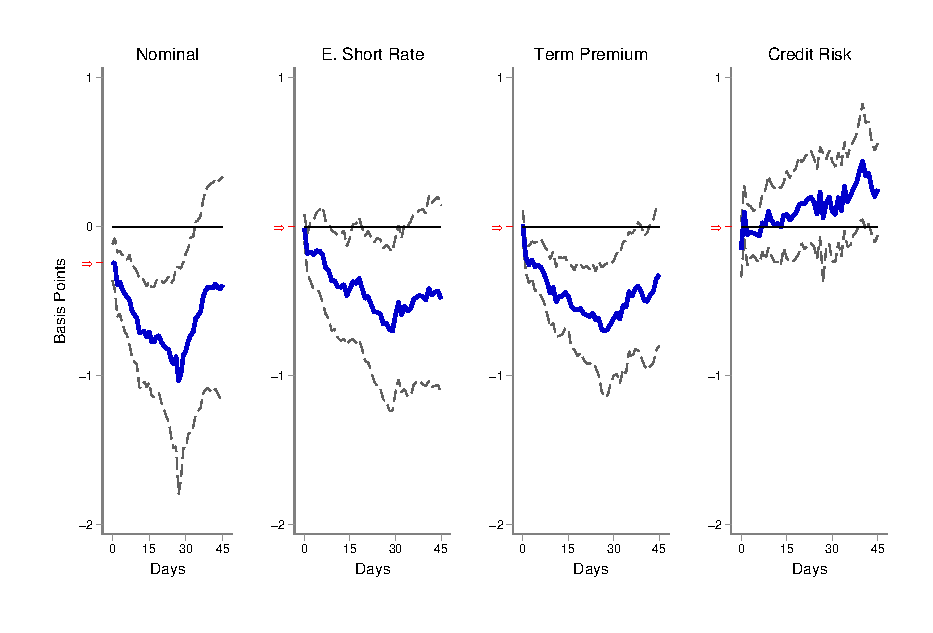
\includegraphics[trim={0cm 0cm 0cm 0cm},clip,height=0.35\textheight,width=\linewidth]{../Figures/PathEMnomyptpphi120m.eps} \\
							\vspace{-0.35cm}
							\caption{10-Year Yield} \label{subfig:LPEM10YpathWh}
						\end{subfigure}
						
						\vspace{0.2cm}
						
						\begin{subfigure}[t]{\linewidth}
							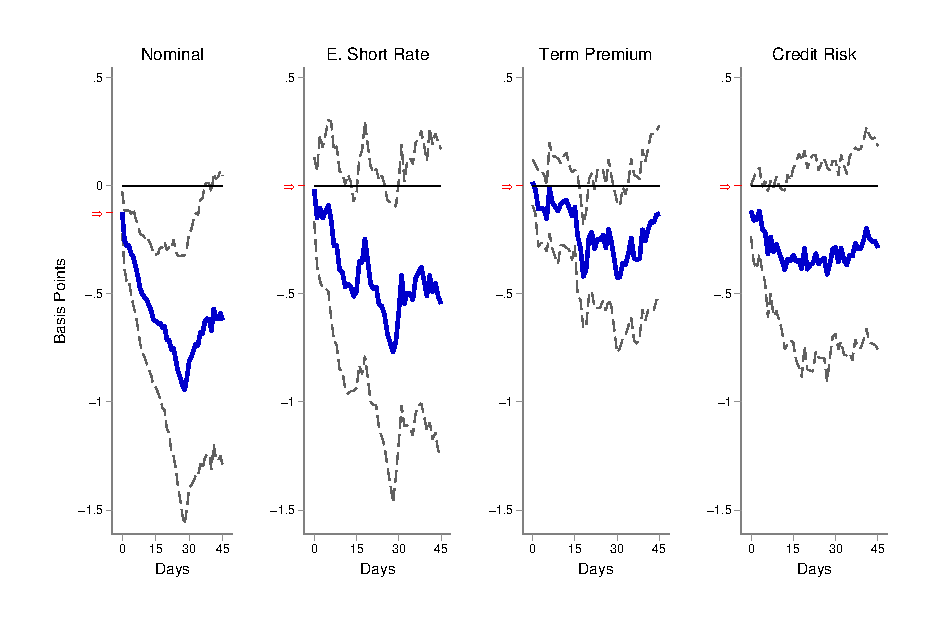
\includegraphics[trim={0cm 0cm 0cm 0cm},clip,height=0.35\textheight,width=\linewidth]{../Figures/PathEMnomyptpphi24m.eps} \\
							\vspace{-0.35cm}
							\caption{2-Year Yield} \label{subfig:LPEM2YpathWh}
						\end{subfigure}
						\vspace{-0.45cm}
					\end{center}
					\fignotes{This figure shows the response of the 10- and 2-year emerging market nominal yields and their components to a forward guidance easing surprise of 1 basis point. Nominal yields are decomposed into an expected future short-term interest rate, a term premium and credit risk compensation, see section \ref{sec:Decomposition} for details. Forward guidance surprises are identified using intraday data around U.S. monetary policy announcements, see section \ref{sec:USMPS} for details. The 90\% confidence bands are based on Driscoll--Kraay standard errors.}
				\end{minipage}
			\end{center}
		\end{figure}
		
	\end{landscape}
	
	
	\begin{figure}[tbph]
		\caption{Response of the Forward Premium to U.S. Monetary Policy Surprises} \label{fig:LPEMRHO}
		\begin{center}
			\begin{minipage}{\linewidth}
				\begin{center}
					\begin{subfigure}[t]{\linewidth}
						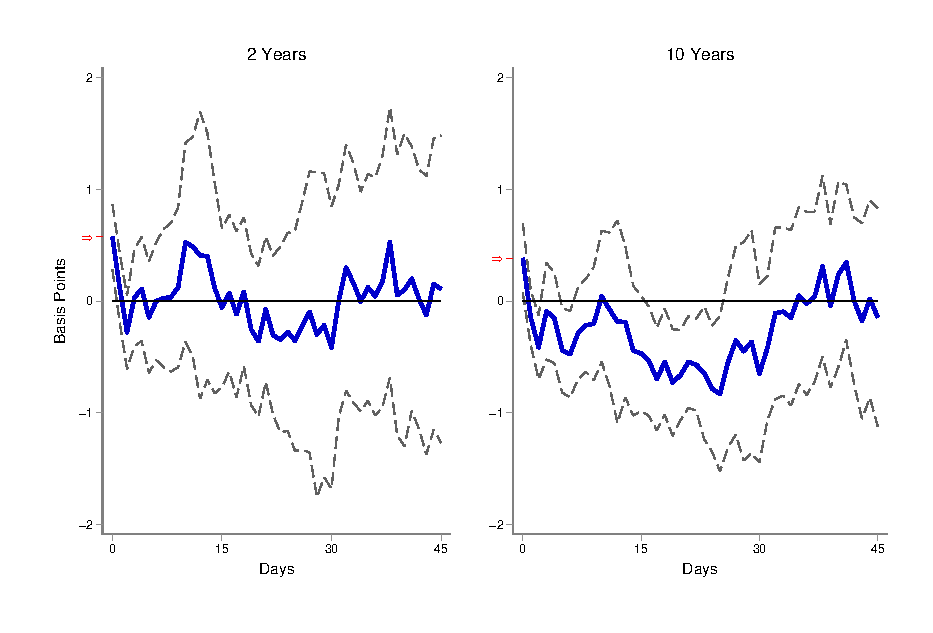
\includegraphics[trim={0cm 0cm 0cm 0cm},clip,height=0.235\textheight,width=\linewidth]{../Figures/TargetEMrho.eps} \\
						\vspace{-0.35cm}
						\caption{Target Surprise: 2000-2008} \label{subfig:LPEMRHOtarget}
					\end{subfigure}
					
					\begin{subfigure}[t]{\linewidth}
						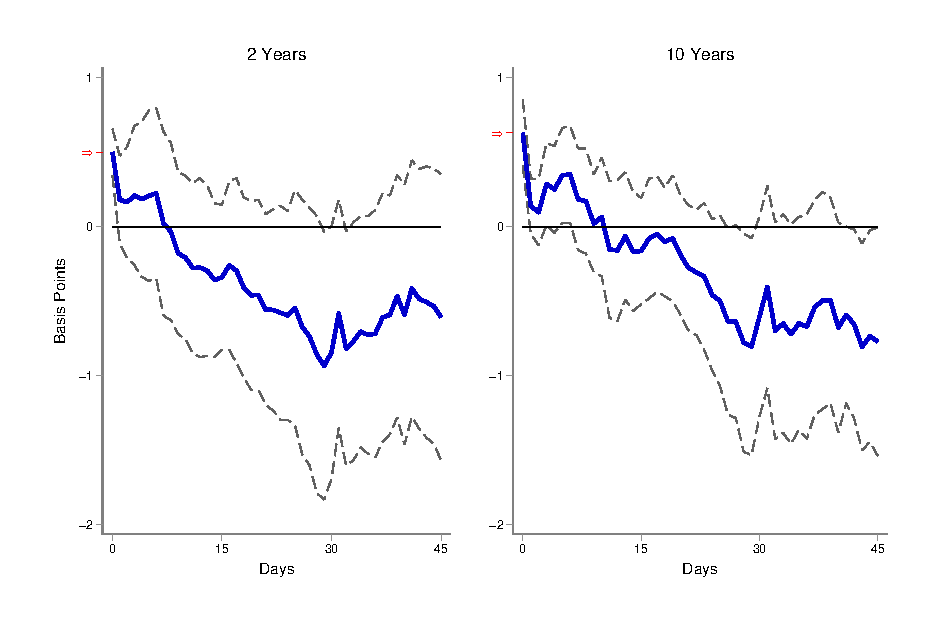
\includegraphics[trim={0cm 0cm 0cm 0cm},clip,height=0.235\textheight,width=\linewidth]{../Figures/PathEMrho.eps} \\
						\vspace{-0.35cm}
						\caption{Forward Guidance Surprise: 2000-2019} \label{subfig:LPEMRHOpath}
					\end{subfigure}
					
					\begin{subfigure}[t]{\linewidth}
						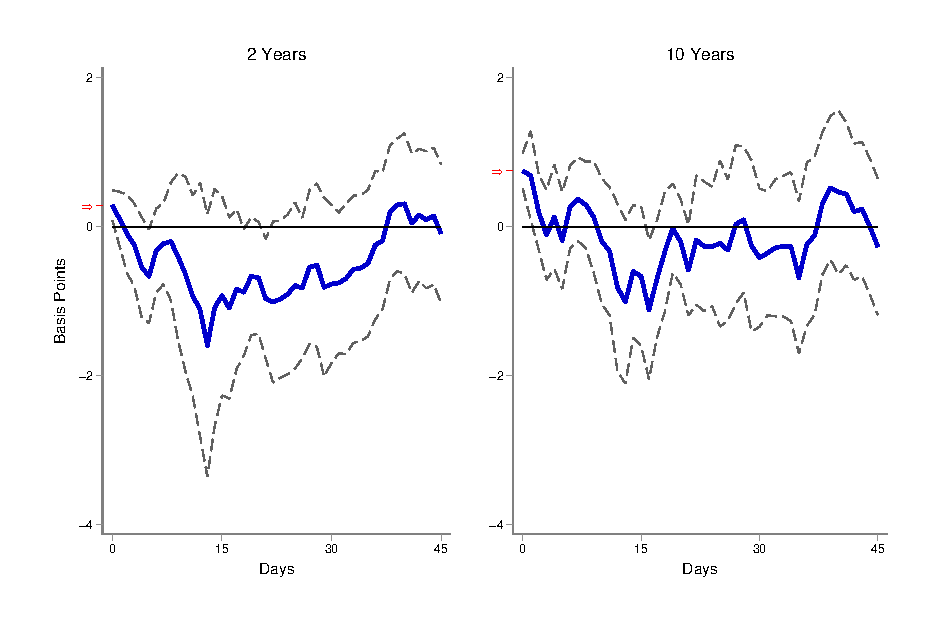
\includegraphics[trim={0cm 0cm 0cm 0cm},clip,height=0.235\textheight,width=\linewidth]{../Figures/LSAPEMrho.eps} \\
						\vspace{-0.35cm}
						\caption{Asset Purchase Surprise: 2009-2019} \label{subfig:LPEMRHOlsap}
					\end{subfigure}
				\end{center}
				\fignotes{This figure shows the response of the 10- and 2-year foreign exchange forward premium of emerging markets to easing surprises in U.S. monetary policy of 1 basis point. The forward premium is calculated using cross-currency swaps, which are in turn constructed using cross-currency basis swaps and interest rate swaps, see section \ref{sec:YCsynt} for details. The target, forward guidance and asset purchase surprises are identified using intraday data around U.S. monetary policy announcements, see section \ref{sec:USMPS} for details. The 90\% confidence bands are based on Driscoll--Kraay standard errors.}
			\end{minipage}
		\end{center}
	\end{figure}
	
	
	\begin{landscape}
		\newpage
	\end{landscape}
	
\end{appendices}

\newpage
\bibliographystyle{abbrvnat} 					% Other styles: plain, authordate1, abbrvnat
	\bibliography{library}

\end{document}